\documentclass[10pt,xcolor=svgnames]{beamer}
\usefonttheme{professionalfonts}
\usepackage[utf8]{inputenc}
\usepackage[T1]{fontenc}
\usepackage[french,english]{babel}
\usepackage{graphicx}
\usepackage{caption,subcaption}
\usepackage{multirow}
\captionsetup{compatibility=false}

\usepackage[style=authoryear,maxbibnames=99,maxcitenames=5,backref=true,backend=biber,citestyle=authoryear]{biblatex}
\AtBeginBibliography{\footnotesize}
\addbibresource{main.bib}

\usepackage[linesnumbered,commentsnumbered,ruled,vlined]{algorithm2e}
\usepackage[linewidth=2.5pt,linecolor=black,nobreak=true]{mdframed}
\mdfsetup{frametitlealignment=\center}

\usepackage{amstext,amsmath,amssymb,bm,bbm,graphicx,mathtools,accents}
\usepackage{beamerleanprogress}
\usepackage{tikz}
\usetikzlibrary{decorations.pathreplacing}
\usepackage{transparent}

%%%%%%%  Environments  %%%%%%%%%%%

\newcounter{definition}[section]
\newenvironment{definition}[1]{\refstepcounter{definition} \par\bigskip \noindent  \begin{minipage}[b]{\linewidth} 
\textbf{Definition~\thedefinition(#1):}}{\end{minipage} \par\bigskip}

\newcounter{example}[section]
\newenvironment{example}{\refstepcounter{example} \par\medskip
\noindent  \begin{minipage}[b]{\linewidth} \textbf{Example~\theexample :}}{\end{minipage} \par\bigskip}

\newcounter{proposition}[section]
\newenvironment{proposition}[1]{\refstepcounter{proposition} \par\medskip \noindent  \begin{minipage}[b]{\linewidth} \textbf{Proposition~\theproposition(#1):}}{\end{minipage} \par\bigskip}

\newcounter{theorem}[section]
\newenvironment{theorem}[1]{\refstepcounter{theorem} \par\medskip \noindent  \begin{minipage}[b]{\linewidth} \textbf{Theorem~\thetheorem(#1):}}{\end{minipage} \par\bigskip}

\newenvironment{proof}{\noindent\ignorespaces\textit{Proof: }}{\hfill $\blacksquare$ \par\noindent\ignorespacesafterend\medskip}

\newcounter{assumption}[section]
\newenvironment{assumption}{ \refstepcounter{assumption} \renewcommand{\theequation}{A.\arabic{assumption}}}{\renewcommand{\theequation}{\arabic{section}.\arabic{equation}} }



%%%%%%%%%%%%%% Commands %%%%%%%%%%%
\newcommand{\daniel}[1]{{\color{black}{#1}}}
\newcommand{\revision}[1]{{\color{blue}{#1}}}

\newcommand{\transp}{\mathbf{T}}
\newcommand{\edge}[2]{ ( #1,#2 )}

\newcommand{\sketch}[1]{{\color{red}{#1}}}
\newcommand{\ol}[1]{{\overline{#1}}}
\newcommand{\av}[1]{\accentset{\circ}{\vec{#1}}}
\newcommand{\Ds}{D}
\newcommand\figTable[2]{\raisebox{-.5\height}{\includegraphics[scale=#1]{#2}}}


\DeclareMathOperator*{\argmin}{arg\,min}
\DeclareMathOperator*{\argmax}{arg\,max}
\renewcommand{\vec}[1]{\bm{#1}}
\DeclarePairedDelimiter\norm{\lVert}{\rVert}%
\DeclarePairedDelimiter\bignorm{\Big\lVert}{\Big\rVert}%
\DeclarePairedDelimiter\abs{\lvert}{\rvert}%

\newcommand{\GG}{ \mathcal{G}_{\vec{I}} }
\newcommand{\GGe}{ \mathcal{G}_{\vec{I}+} }
\newcommand{\GGc}[1]{ \mathcal{G}_C^{(#1)} }
\newcommand{\GGcc}{ \mathcal{G}_C}

\makeatletter
\DeclareFontFamily{U}{tipa}{}
\DeclareFontShape{U}{tipa}{m}{n}{<->tipa10}{}
\newcommand{\arc@char}{{\usefont{U}{tipa}{m}{n}\symbol{62}}}%

\newcommand{\arc}[1]{\mathpalette\arc@arc{#1}}

\newcommand{\arc@arc}[2]{%
  \sbox0{$\m@th#1#2$}%
  \vbox{
    \hbox{\resizebox{\wd0}{\height}{\arc@char}}
    \nointerlineskip
    \box0
  }%
}
\makeatother


%%%%%%%%%%% Misc %%%%%%%%%%%
\crefname{algocf}{alg.}{algs.}
\Crefname{algocf}{Algorithm}{Algorithms}
\Crefname{appsec}{Appendix}{Appendices}  

\setbeamertemplate{bibliography entry title}{}
\setbeamertemplate{bibliography entry location}{}
\setbeamertemplate{bibliography entry note}{}

\tikzset{
  invisible/.style={opacity=0},
  visible on/.style={alt={#1{}{invisible}}},
  alt/.code args={<#1>#2#3}{%
    \alt<#1>{\pgfkeysalso{#2}}{\pgfkeysalso{#3}} % \pgfkeysalso doesn't change the path
  },
}

\title
  [Max-flow for digital elastica shape optimization]
  {A maximum-flow model for digital elastica shape optimization}

\author[Daniel Martins Antunes et al.]{  
  {Daniel Martins Antunes\textsuperscript{1} , Jacques-Olivier
    Lachaud\textsuperscript{1} \\
    and Hugues Talbot\textsuperscript{2}}
}
  
  
\date
  {CIRM, April 1st 2021}


\institute
  {
	\textsuperscript{1}LAMA, Université Savoie Mont Blanc \\ 
	\textsuperscript{2}CentraleSupélec, Université Paris-Saclay
  }
 
\begin{document}
  \maketitle
  \captionsetup[subfigure]{labelformat=empty}

\begin{frame}
	{Outline}

\begin{enumerate}
	\item{Motivation}
	\begin{itemize}
		\item{Image analysis and geometric priors}
		\item{Elastica model and completion property}		
		\item{State-of-the-art}							
	\end{itemize}
      \vspace{1em}
	{\transparent{0.4}
	\item{Contribution}
	\begin{itemize}
		\item{Digital sets and convergent estimators}		
		\item{(A combinatorial model for elastica)}
		\item{(A quadratic non-submodular formulation for elastica)}	
		\item{Elastica minimization via graph-cuts}	
	\end{itemize}}
	\vspace{1em}
	\item{Conclusion and perspectives}
\end{enumerate}
\end{frame}

\section{Motivation}

\begin{frame}
	{Motivation}	
	{Image analysis}

\begin{minipage}[t][0.5\textheight][t]{1\textwidth}
The problems we are interested in come from \emph{image analysis}.
\vspace{1em}

\only<1-4>{
\begin{center}
\begin{tabular}{ccc}
\highlight{2}{1,3-}{\textbf{Segmentation}} & 
\highlight{3}{1-2,4-}{\textbf{Denoising}} & 
\highlight{4}{1-3,5-}{\textbf{Inpainting}}
\end{tabular}
\end{center}}

\only<2>{
\center
\begin{tabular}{p{0.4\textwidth}c}
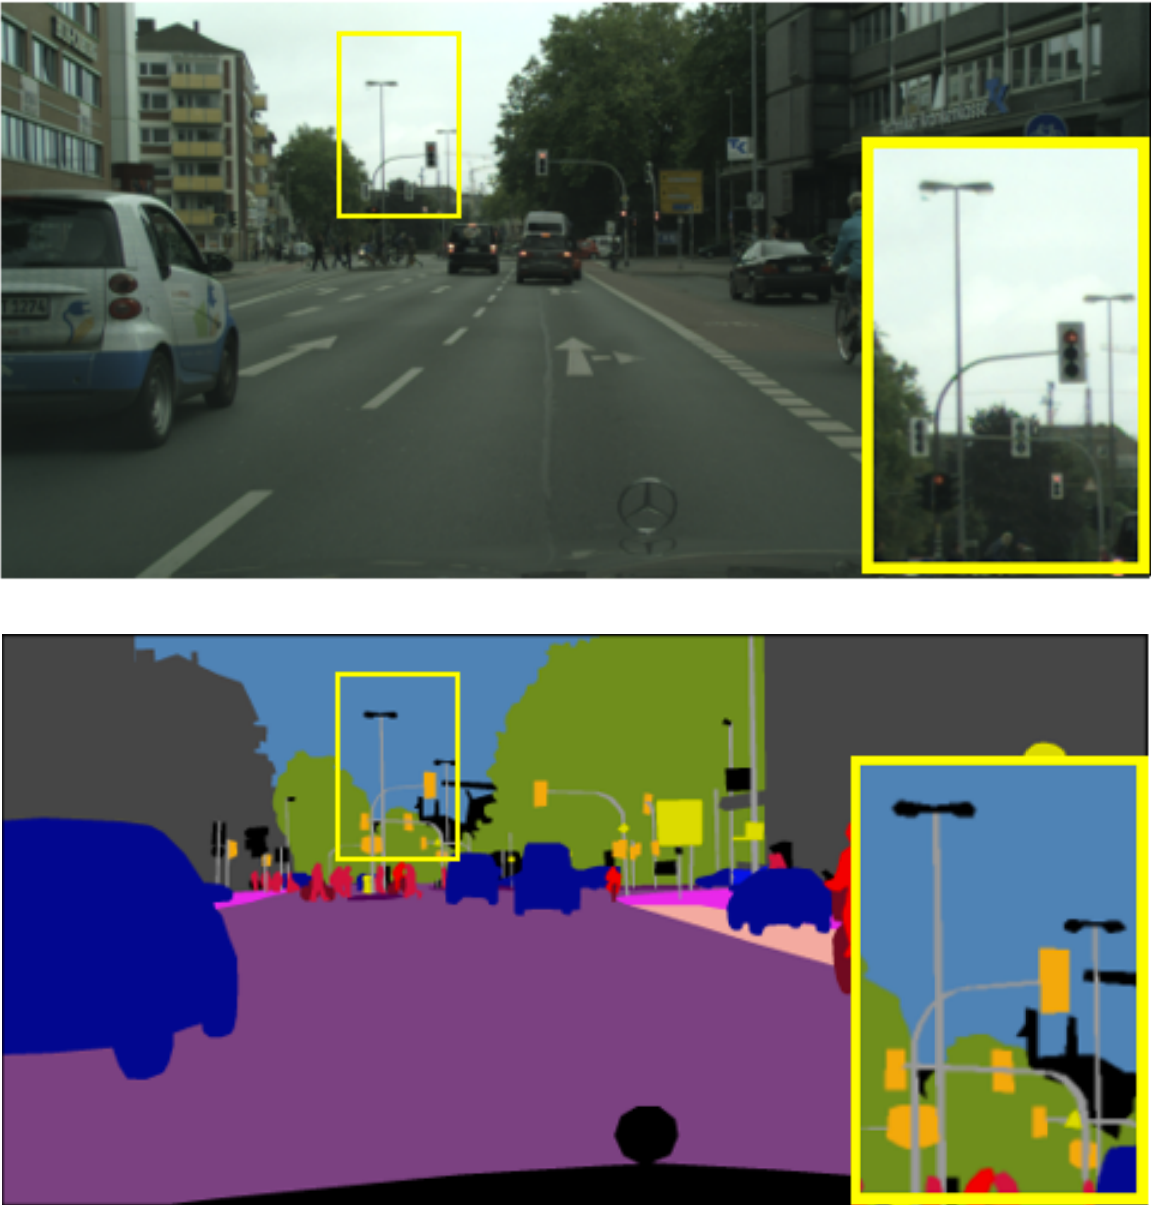
\includegraphics[scale=0.4]{figures/motivation/image-analysis/segmentation-cars.png} &
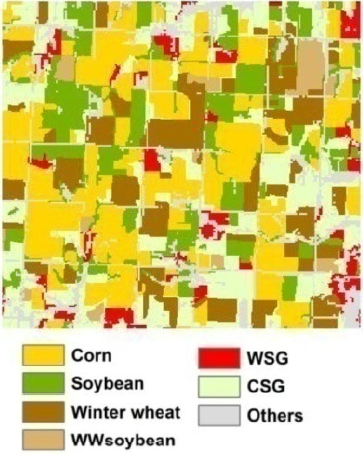
\includegraphics[scale=0.4]{figures/motivation/image-analysis/segmentation-crops.png}\\
\mycite{li2019gff} & \mycite{li2015object}
\end{tabular}}%
\only<3>{
\center
\begin{tabular}{cc}
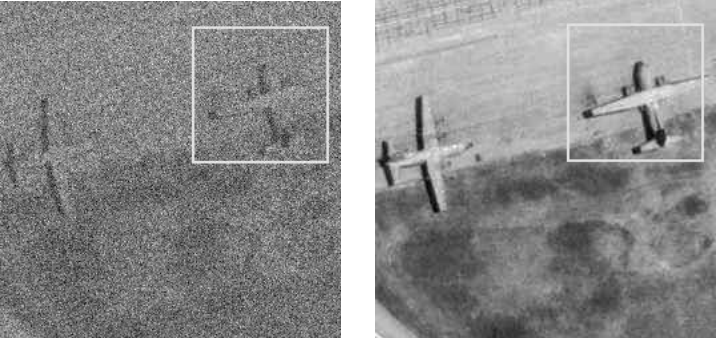
\includegraphics[scale=0.44]{figures/motivation/image-analysis/denoising-airplane.png} &
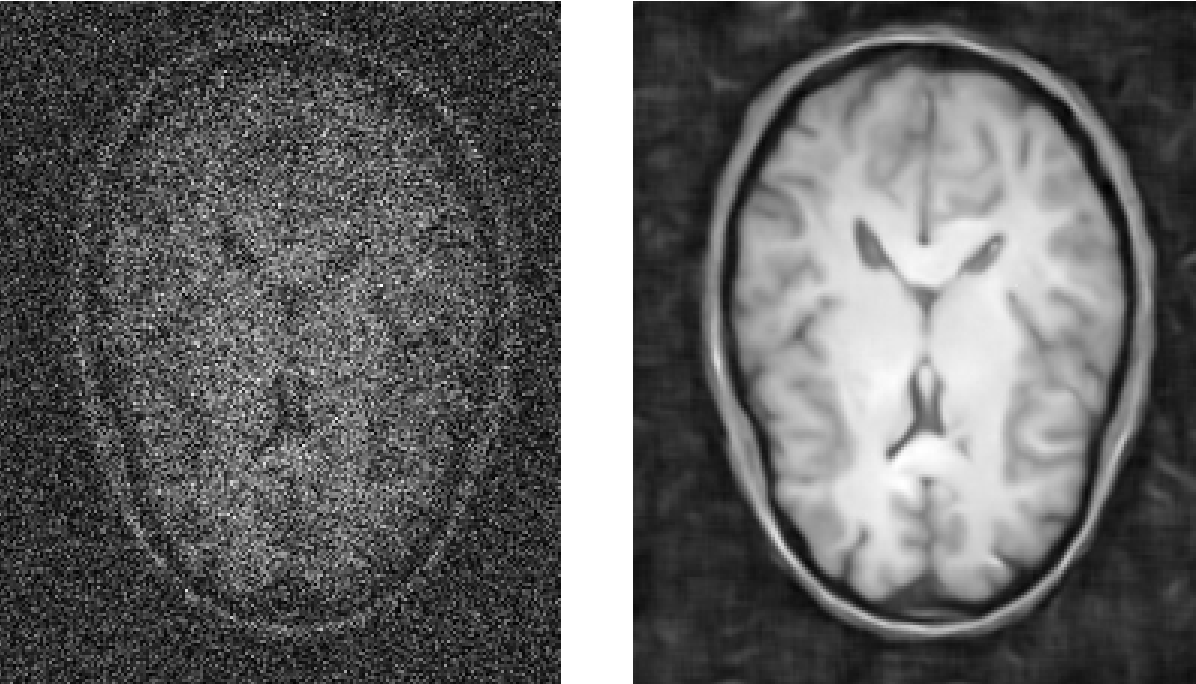
\includegraphics[scale=0.22]{figures/motivation/image-analysis/denoising-mri.png} \\
\mycite{xu2018deep} & \mycite{jiang2018denoising}
\end{tabular}}%
\only<4>{
\center
\begin{tabular}{cc}
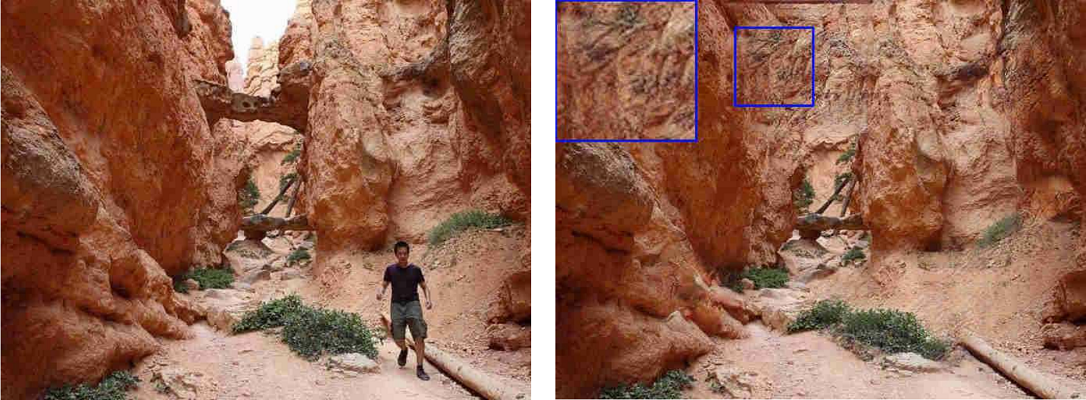
\includegraphics[scale=0.3]{figures/motivation/image-analysis/inpainting-man.png} &
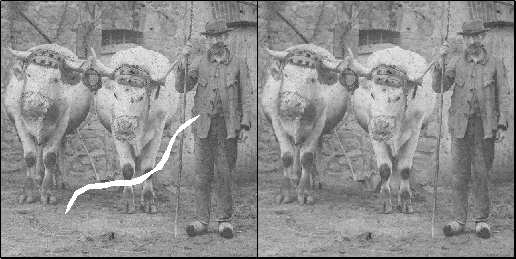
\includegraphics[scale=0.24]{figures/motivation/image-analysis/inpainting-picture.png} \\
\mycite{yu2018generative} &  \mycite{masnou98inpainting}
\end{tabular}}%
\only<5->{
\begin{tabular}{p{0.6\textwidth}p{0.2\textwidth}}
\textbf{Segmentation:} $\mathcal{I}^{\star} = \argmin_{\mathcal{I}} E_{seg}(\mathcal{I},f_{\vec{I}}).$ & \raisebox{-.5\height}{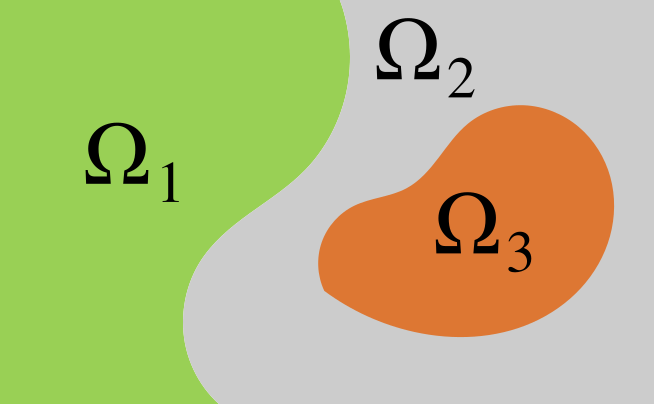
\includegraphics[scale=0.24]{figures/motivation/image-analysis/segmentation-stylised.png}}\\[2em]
\textbf{Denoising:} $f_{\widehat{\vec{I}}} = \argmin_f E_{den}(f,f_{\vec{\widetilde{I}}}).$ & \raisebox{-.5\height}{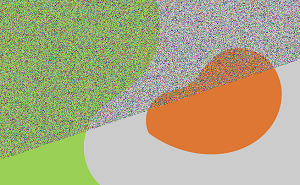
\includegraphics[scale=0.24]{figures/motivation/image-analysis/denoising-stylised.png}}\\[2em]
\textbf{Inpainting:} $f_{\vec{\widehat{I}}} = \argmin_f E_{inp}(f,f_{\widetilde{\vec{I}}}).$ & \raisebox{-.5\height}{
\includegraphics[scale=0.24]{figures/motivation/image-analysis/inpainting-stylised.png}}
\end{tabular}}
\end{minipage}
%6
%
\begin{minipage}[t][0.27\textheight][t]{\textwidth}
\only<5->{We focused on \emph{variational approaches} to solve these problems.}

\only<6->{
Energies are defined by terms that guides the optimization towards solution with special properties e.g.,
\begin{itemize}
	\item{ \emph{Data fidelity}. The solution should not differ much from the input. }
	\item{ \emph{Spatial coherence}. Images are composed of regions with low variability in color. }
\end{itemize}
}
\end{minipage}

\end{frame}







\begin{frame}
{Motivation}
{Geometric priors}
The \emph{Mumford Shah}~(\mycite{mumford89}) is a model for segmentation and denoising.
%
%
\begin{align*}
	\min_{f,\highlight{4}{1-3,5-}{\mathcal{K}}} \alpha \int_{\Omega} \highlight{2}{1,3-}{\norm{ f_{\vec{I}} - f}^2}dx + \beta \int_{\Omega \setminus \highlight{4}{1-3,5-}{\mathcal{K}}} \highlight{3}{1,2,4-}{\norm{ \nabla f}^2} dx + \lambda Per(\highlight{4}{1-3,5-}{\mathcal{K}}).
\end{align*}
%
%
\onslide<5->{
The \emph{ROF}~(\mycite{rudin92}) model uses \emph{total variation} for image denoising.
%
%
\begin{align*}
	\min_{f} \alpha \int_{\Omega} \norm{ f_{\vec{I}} - f}^2dx + \beta \int_{\Omega} \highlight{6}{1-5,7-}{\norm{ \nabla f }}dx.
\end{align*}}
%
%
\onslide<7->{
\begin{itemize}
	\item{A measure of perimeter is present in both models.}
	\item{\emph{Geometric priors} as perimeter, area or curvature are useful due to its flexibility and effect predictability.}
\end{itemize}}
%
%
\vspace{1em}
\onslide<8->{
In this thesis, we are interested in the combined use of \emph{perimeter} and \emph{squared curvature} as geometric priors.}
\end{frame}

\begin{frame}
{Motivation}
{Completion property}
\begin{minipage}[t][0.5\textheight][t]{\textwidth}
\only<1->{
\center
$\min_{ \Omega \in \{\Omega_{c}, \Omega_{d} \} } Perimeter(\Omega).$
}
\only<1>{
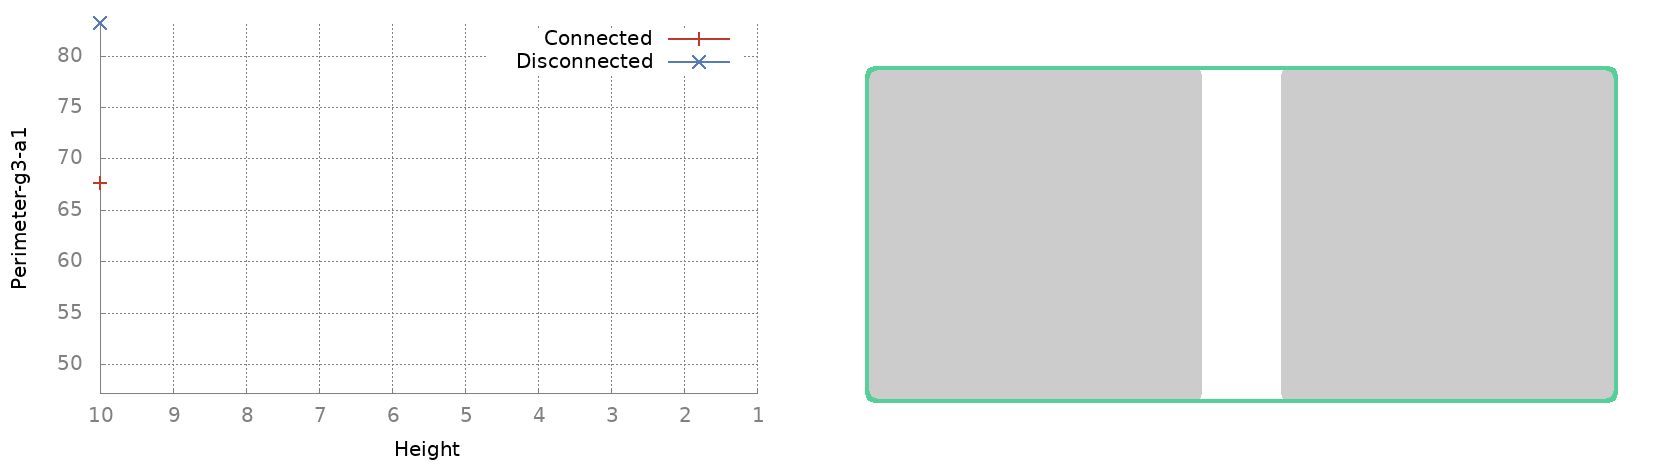
\includegraphics[scale=0.25]{figures/motivation/completion/perimeter-0.png}
}
\only<2>{
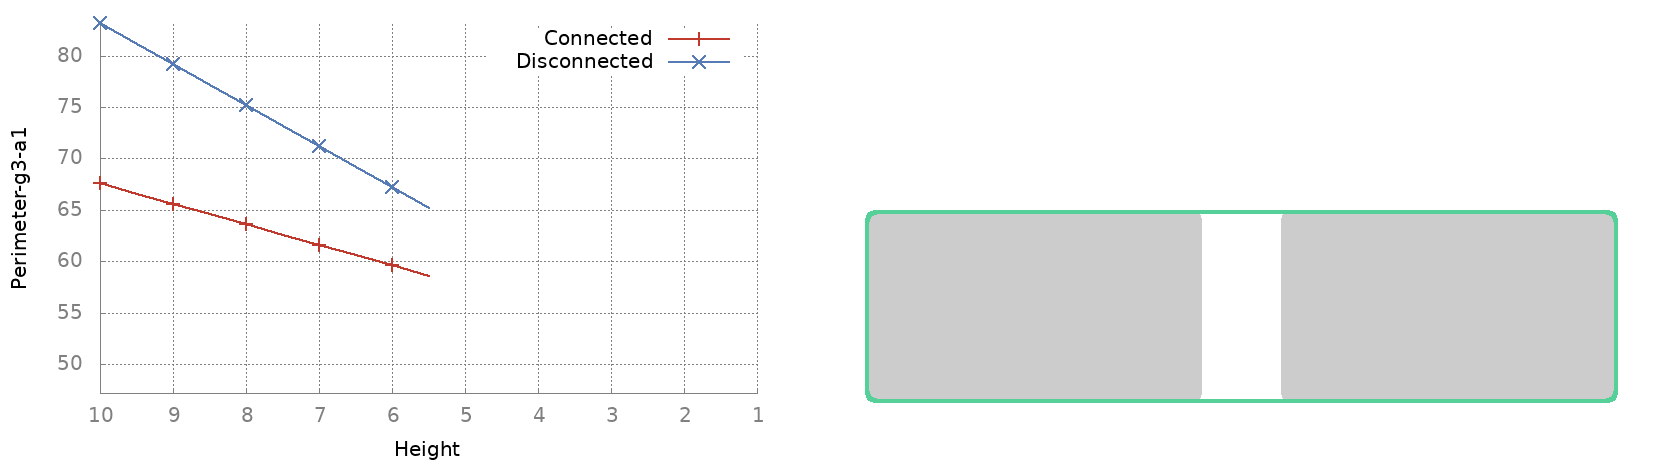
\includegraphics[scale=0.25]{figures/motivation/completion/perimeter-1.png}
}
\only<3>{
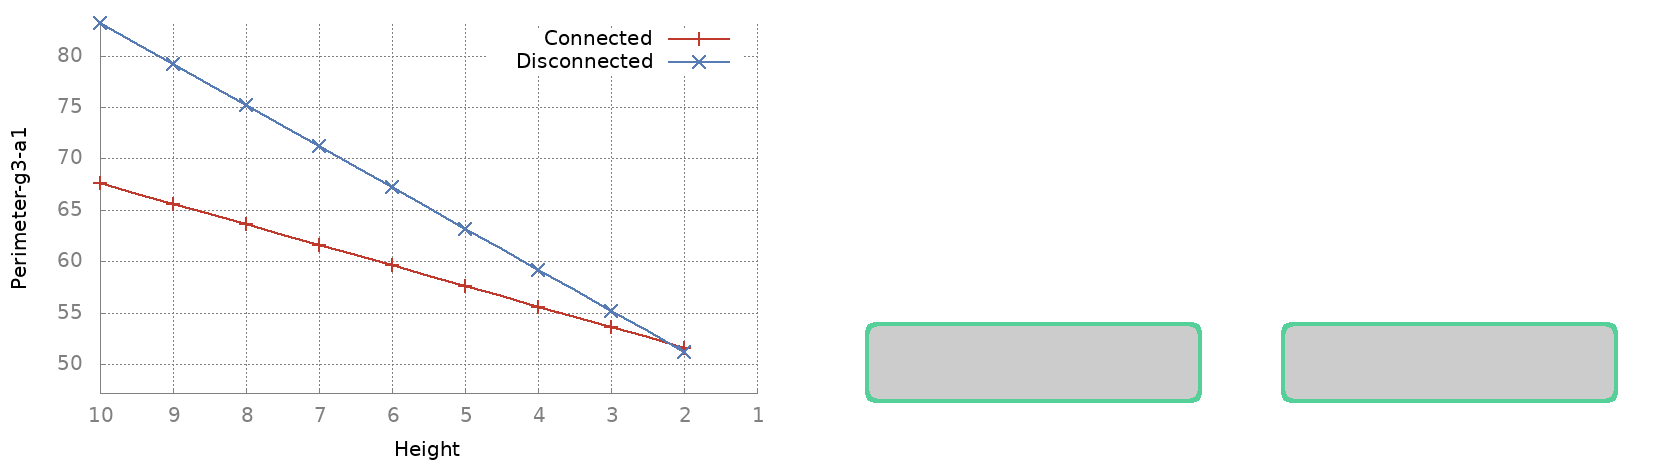
\includegraphics[scale=0.25]{figures/motivation/completion/perimeter-2.png}
}
\only<4->{
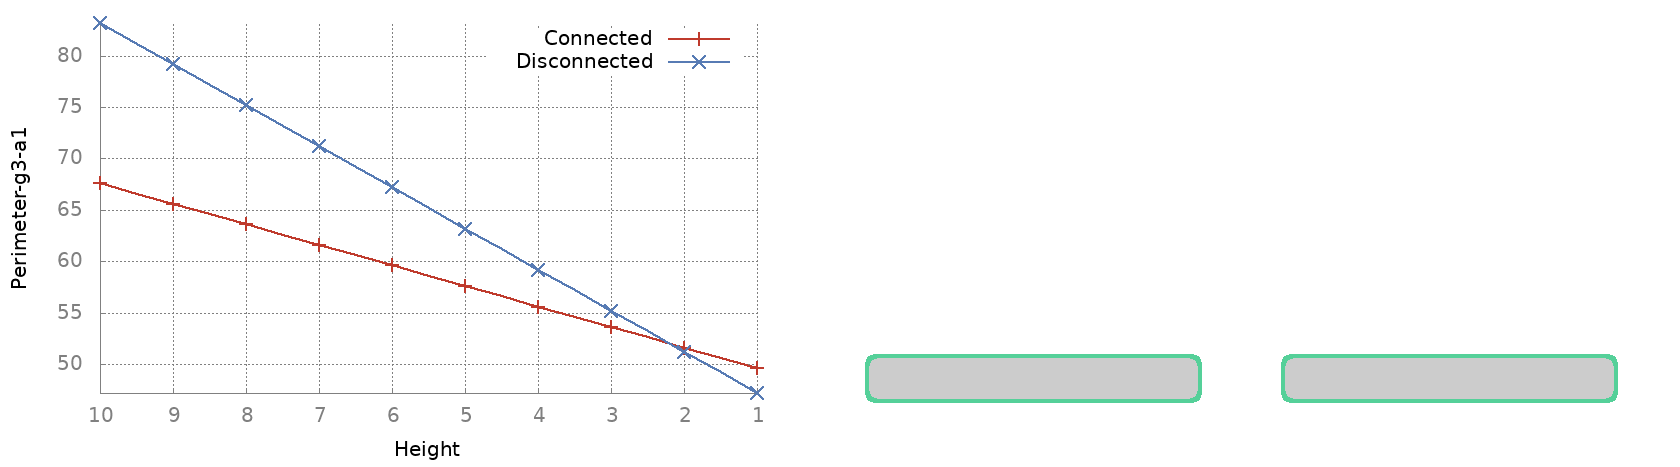
\includegraphics[scale=0.25]{figures/motivation/completion/perimeter-3.png}
}
\end{minipage}
\begin{minipage}[t][0.5\textheight][t]{\textwidth}
\only<5->{
\center
$\min_{ \Omega \in \{\Omega_{c}, \Omega_{d} \} } Perimeter(\Omega) + Squared\;Curvature(\partial \Omega).$}
\only<5>{
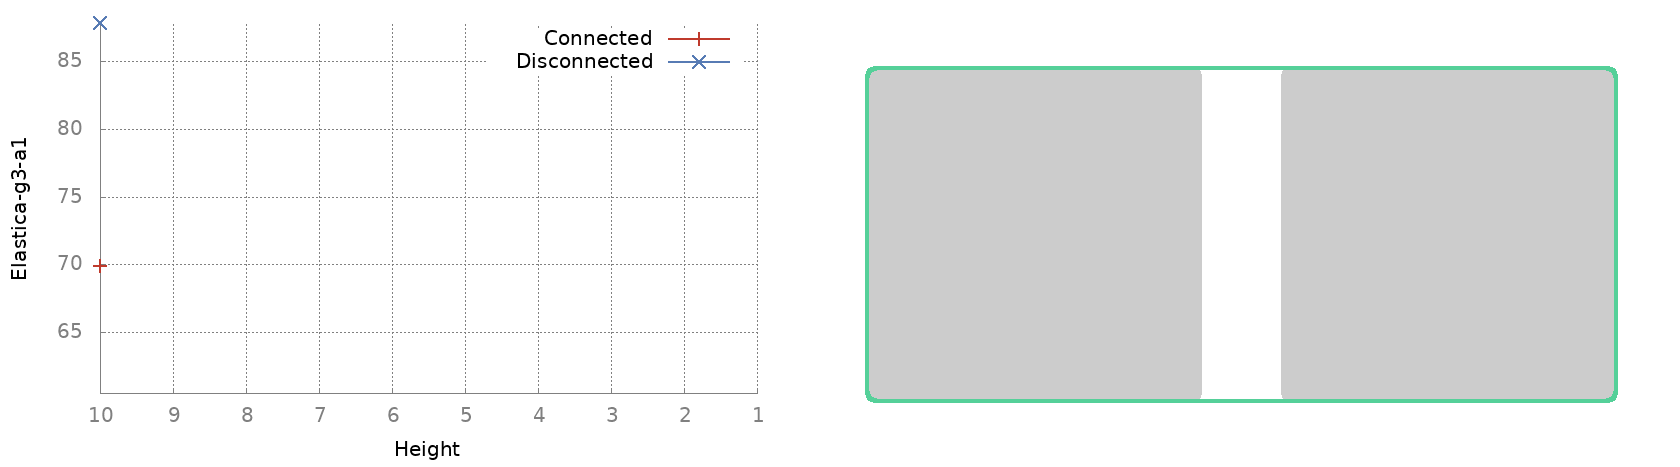
\includegraphics[scale=0.25]{figures/motivation/completion/elastica-0.png}
}
\only<6>{
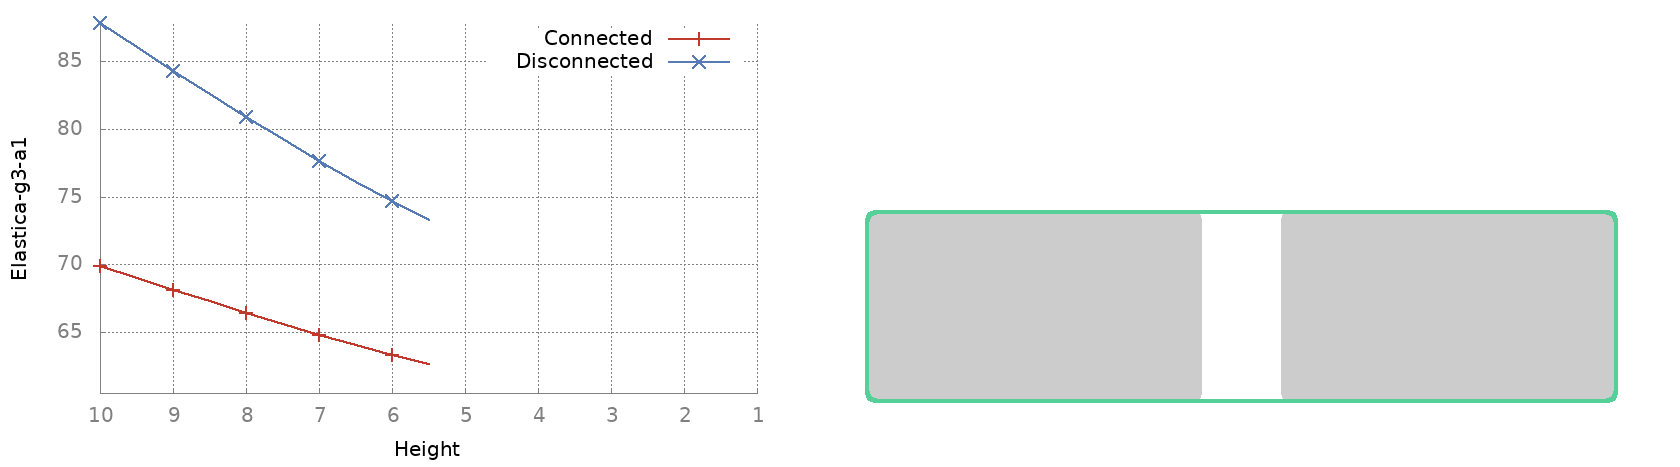
\includegraphics[scale=0.25]{figures/motivation/completion/elastica-1.png}
}
\only<7>{
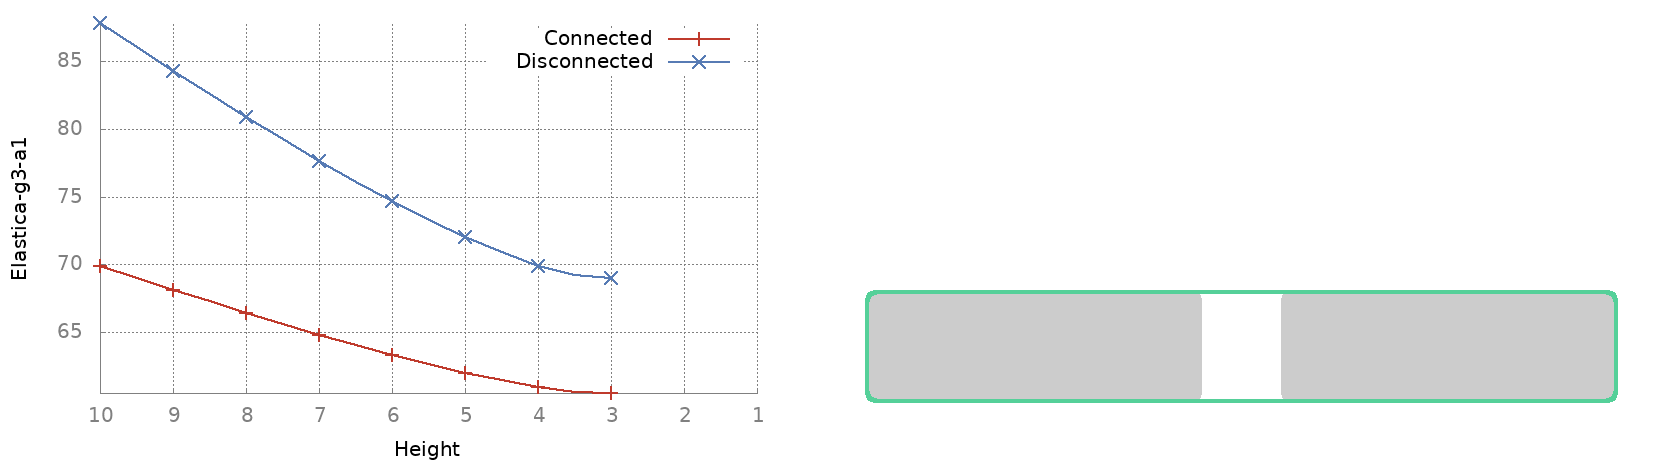
\includegraphics[scale=0.25]{figures/motivation/completion/elastica-2.png}
}
\only<8->{
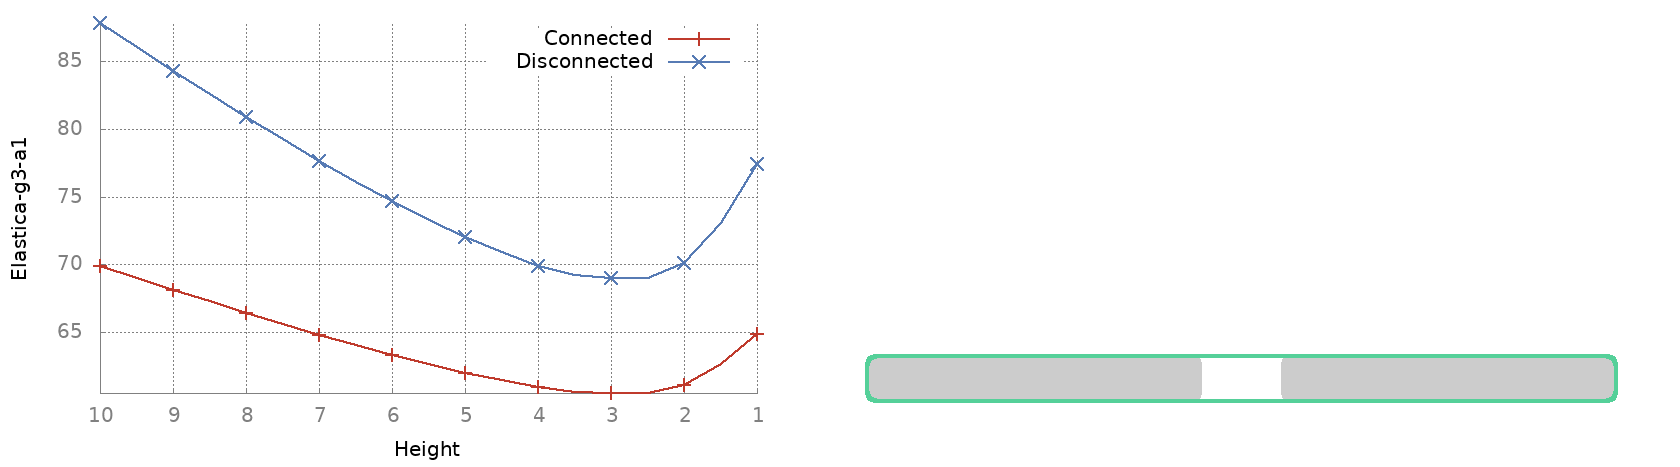
\includegraphics[scale=0.25]{figures/motivation/completion/elastica-3.png}
}
\end{minipage}
\end{frame}

\begin{frame}
{Motivation}
{Completion property}
\begin{minipage}[t][0.5\textheight][t]{\textwidth}
\only<1->{
\center
$\min_{ \Omega \in \{\Omega_{c}, \Omega_{d} \} } Perimeter(\Omega) + Squared\;Curvature(\partial \Omega).$}
\only<1>{
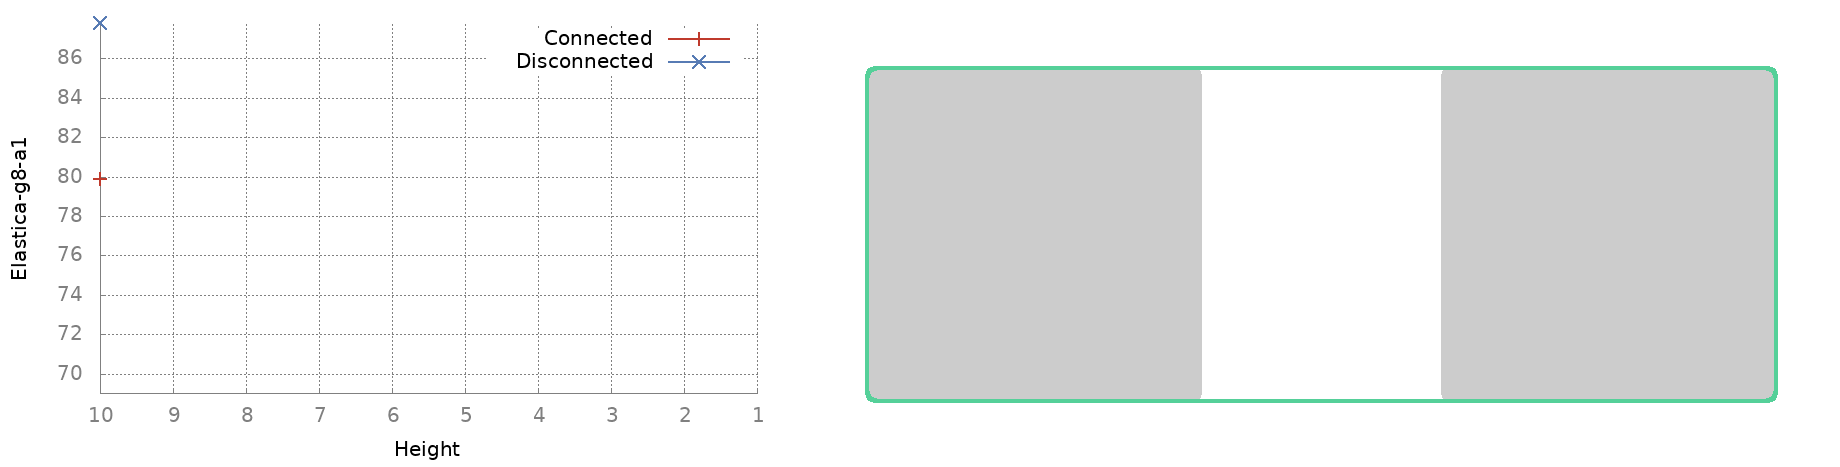
\includegraphics[scale=0.22]{figures/motivation/completion/elastica-g8a1-0.png}
}
\only<2>{
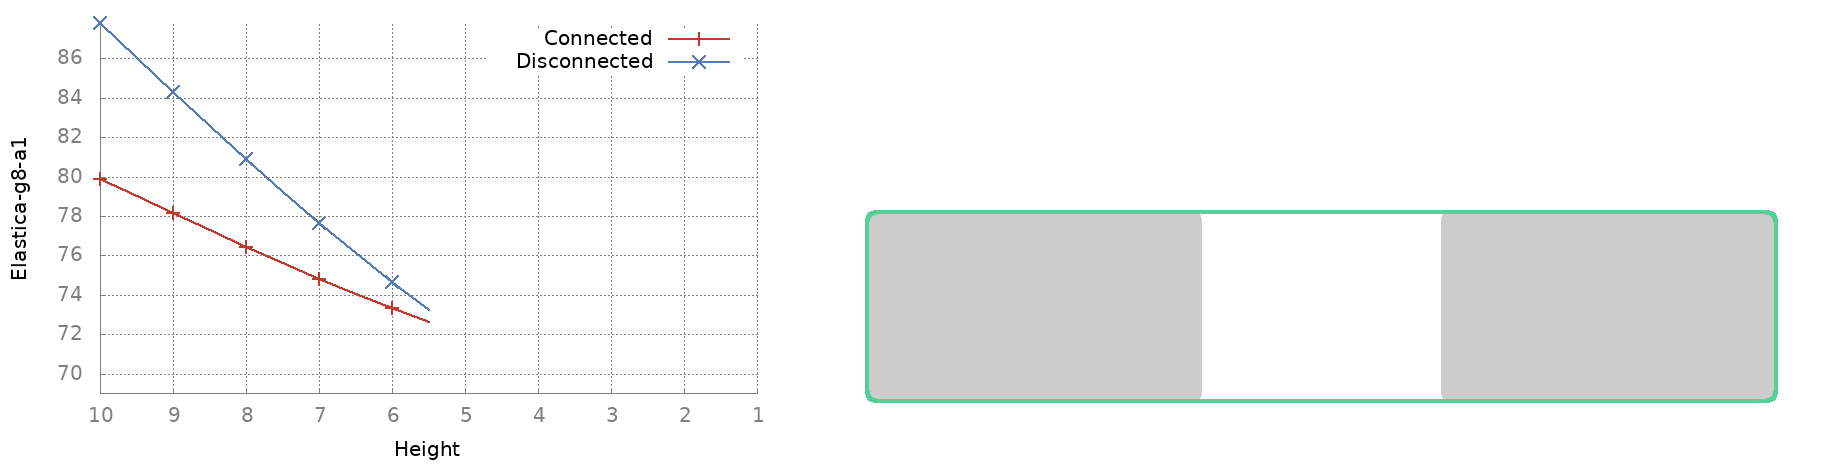
\includegraphics[scale=0.22]{figures/motivation/completion/elastica-g8a1-1.png}
}
\only<3>{
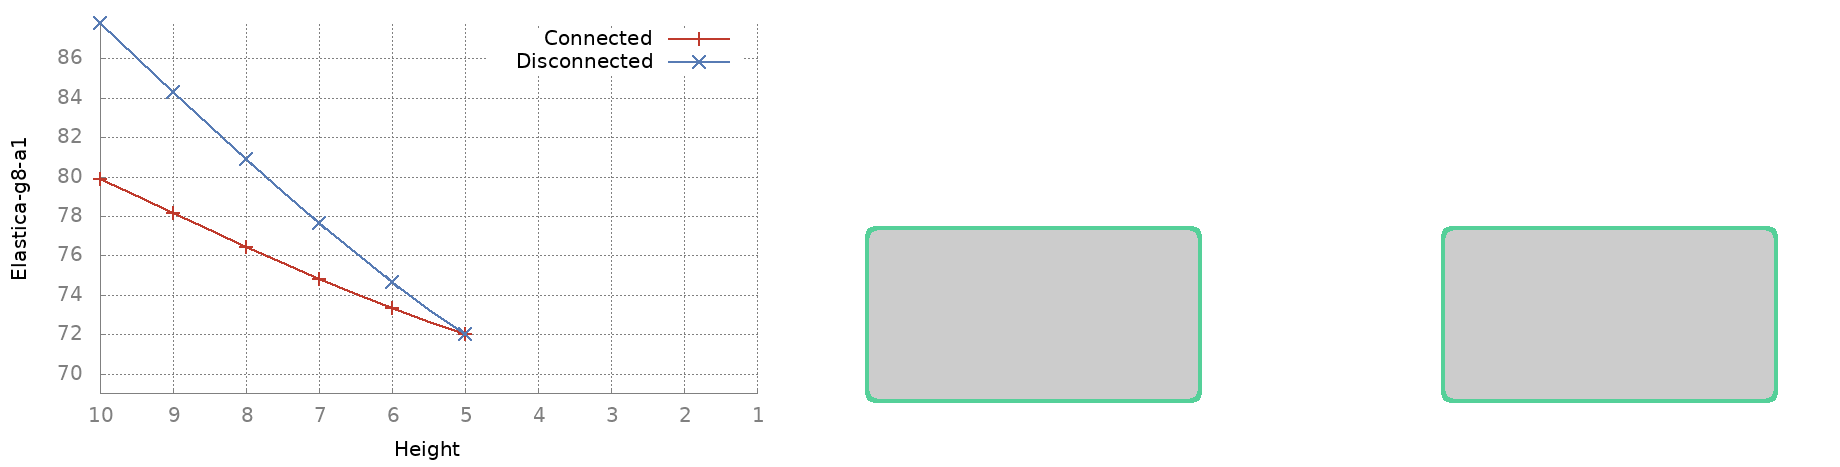
\includegraphics[scale=0.22]{figures/motivation/completion/elastica-g8a1-2.png}
}
\only<4>{
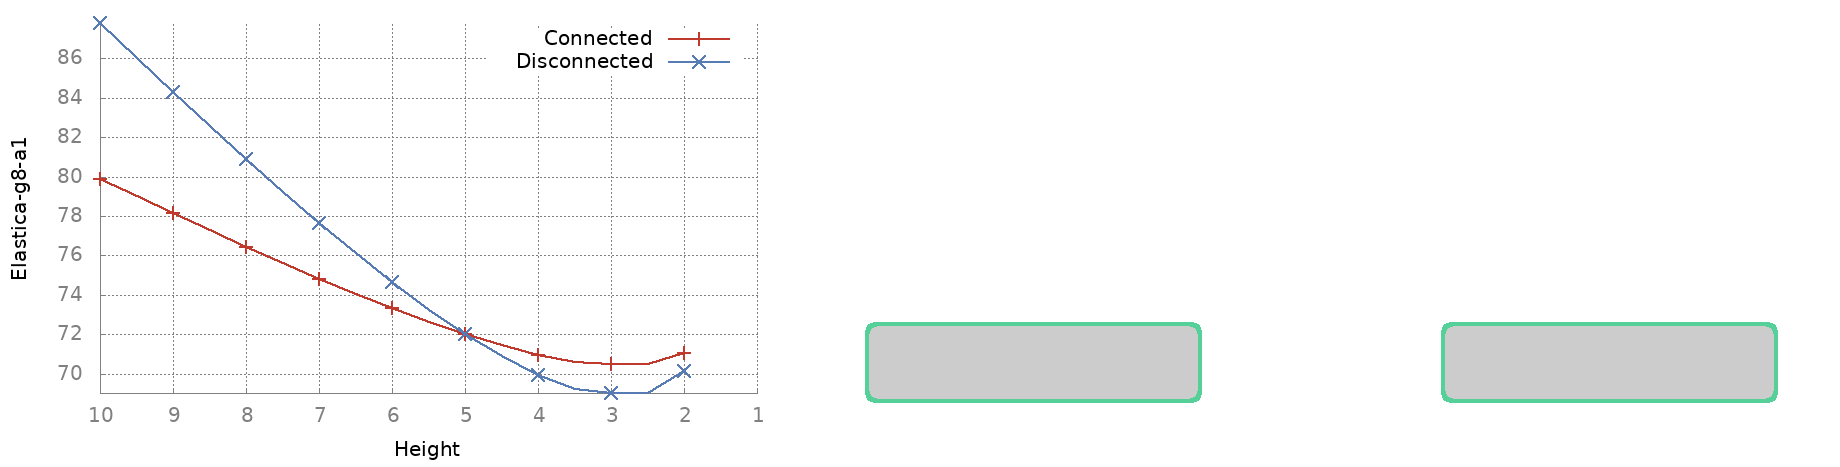
\includegraphics[scale=0.22]{figures/motivation/completion/elastica-g8a1-3.png}
}
\only<5->{
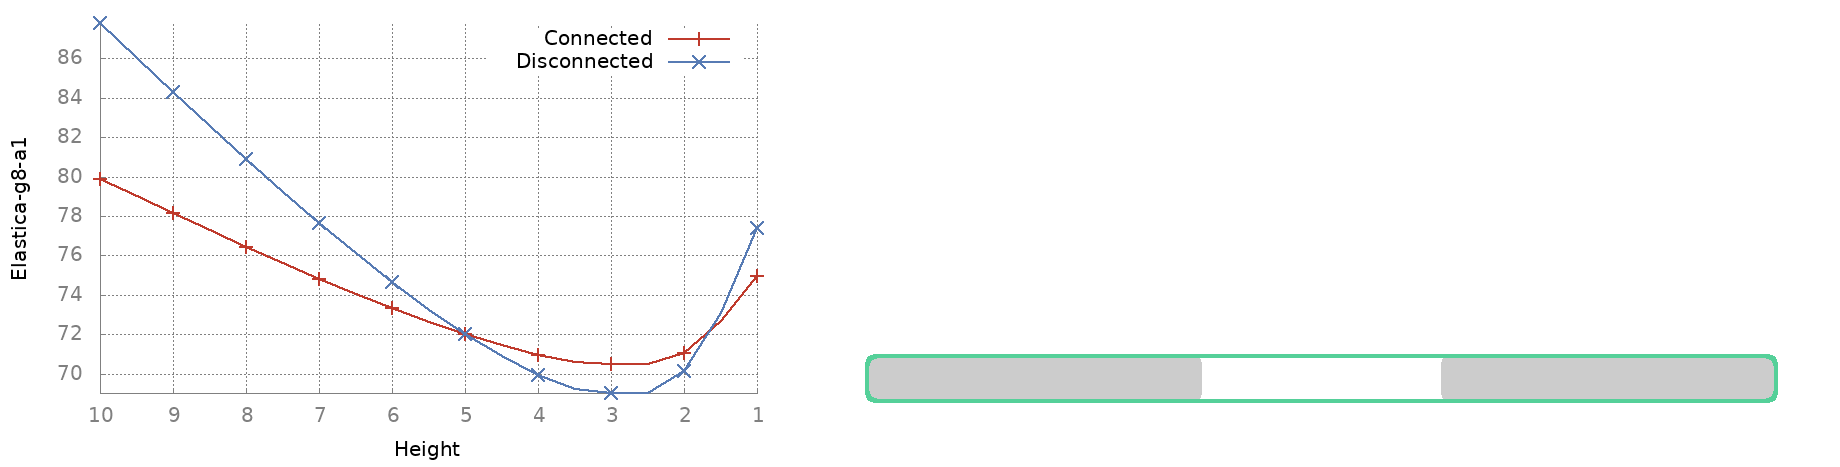
\includegraphics[scale=0.22]{figures/motivation/completion/elastica-g8a1-4.png}
}
\end{minipage}
\begin{minipage}[t][0.5\textheight][t]{\textwidth}
\only<6-9>{
\center
$\min_{ \Omega \in \{\Omega_{c}, \Omega_{d} \} } \frac{1}{2}Perimeter(\Omega) + Squared\;Curvature(\partial \Omega).$}
\only<10->{
\center
\color{highlightcolor} $\min_{ \Omega \in \{\Omega_{c}, \Omega_{d} \} } \int_{\partial \Omega}{ \alpha + \beta \kappa ^2ds}. \quad - \quad \text{The elastica energy}$}
\only<6>{
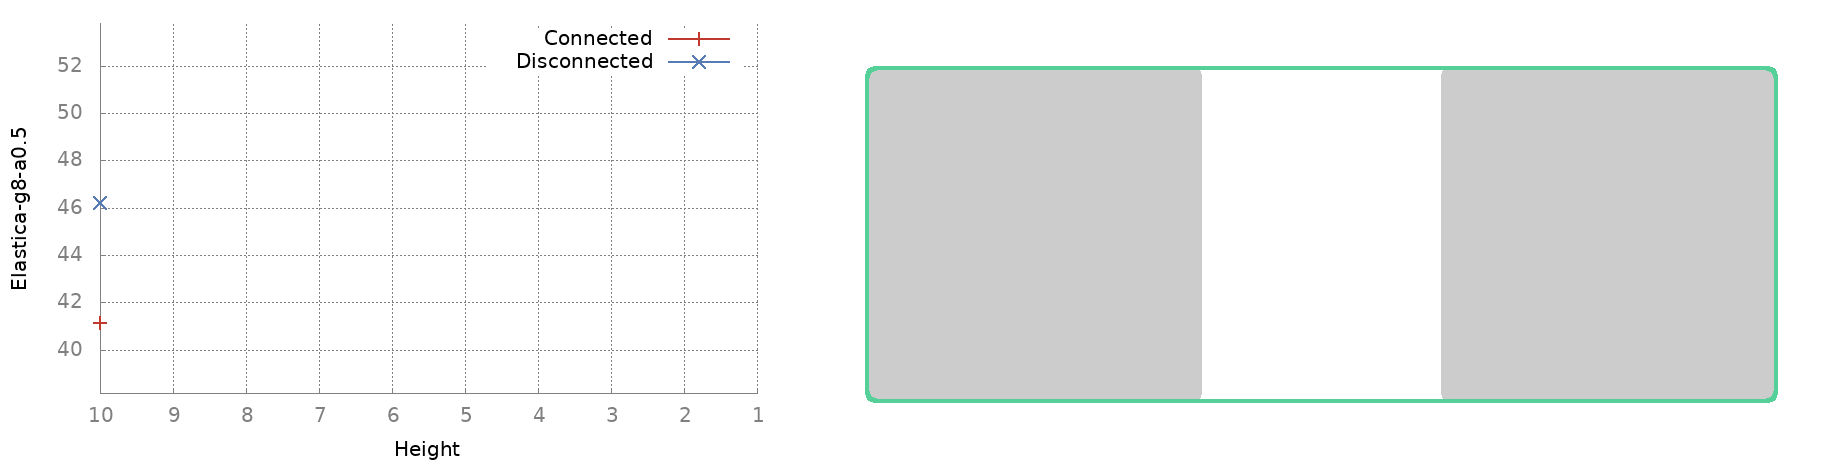
\includegraphics[scale=0.22]{figures/motivation/completion/elastica-g8a05-0.png}
}
\only<7>{
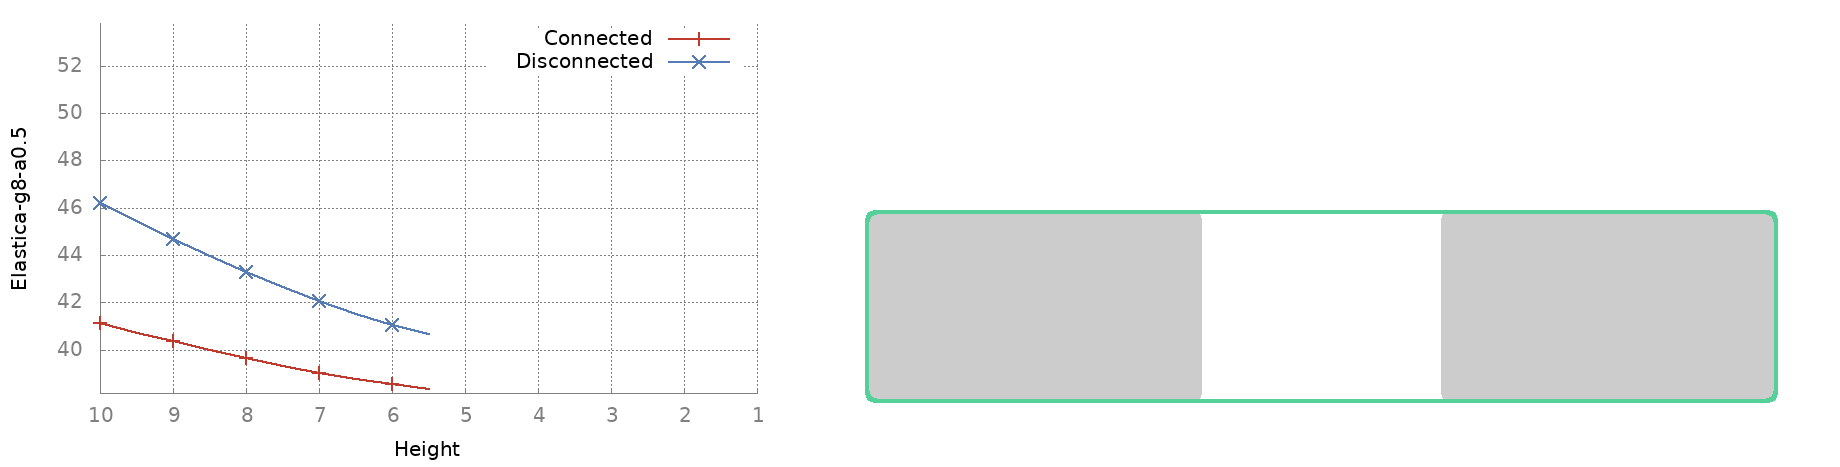
\includegraphics[scale=0.22]{figures/motivation/completion/elastica-g8a05-1.png}
}
\only<8>{
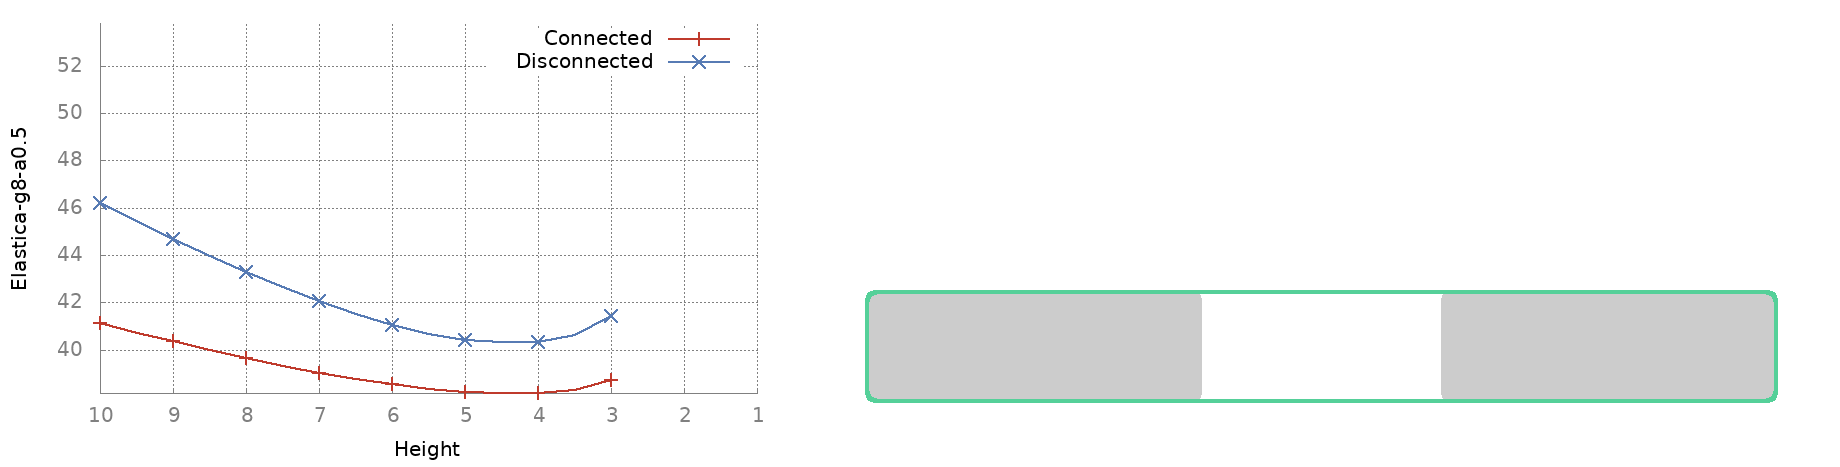
\includegraphics[scale=0.22]{figures/motivation/completion/elastica-g8a05-2.png}
}
\only<9->{
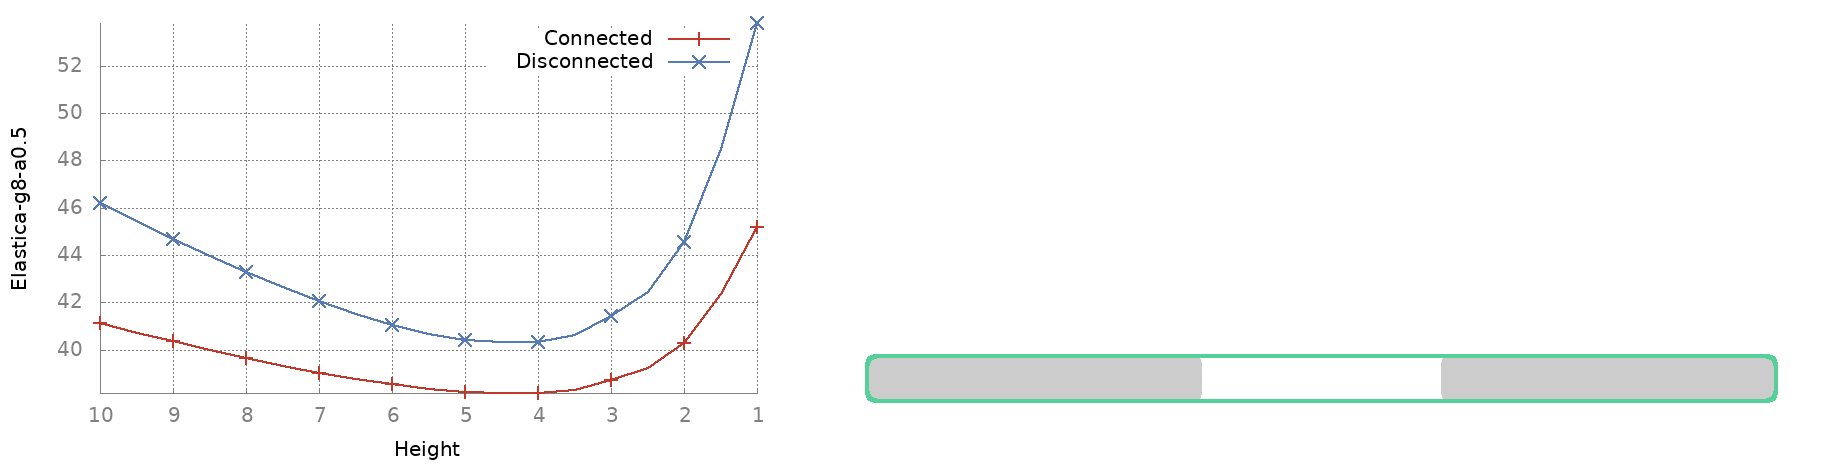
\includegraphics[scale=0.22]{figures/motivation/completion/elastica-g8a05-3.png}
}
\onslide<11>{
	\begin{figure}
	\begin{tikzpicture}[overlay, remember picture] 
	\node at (current page.center) 
	    [
	    anchor=east,
	    xshift=-10mm,
	    yshift=0mm
	    ] 
	{
	
	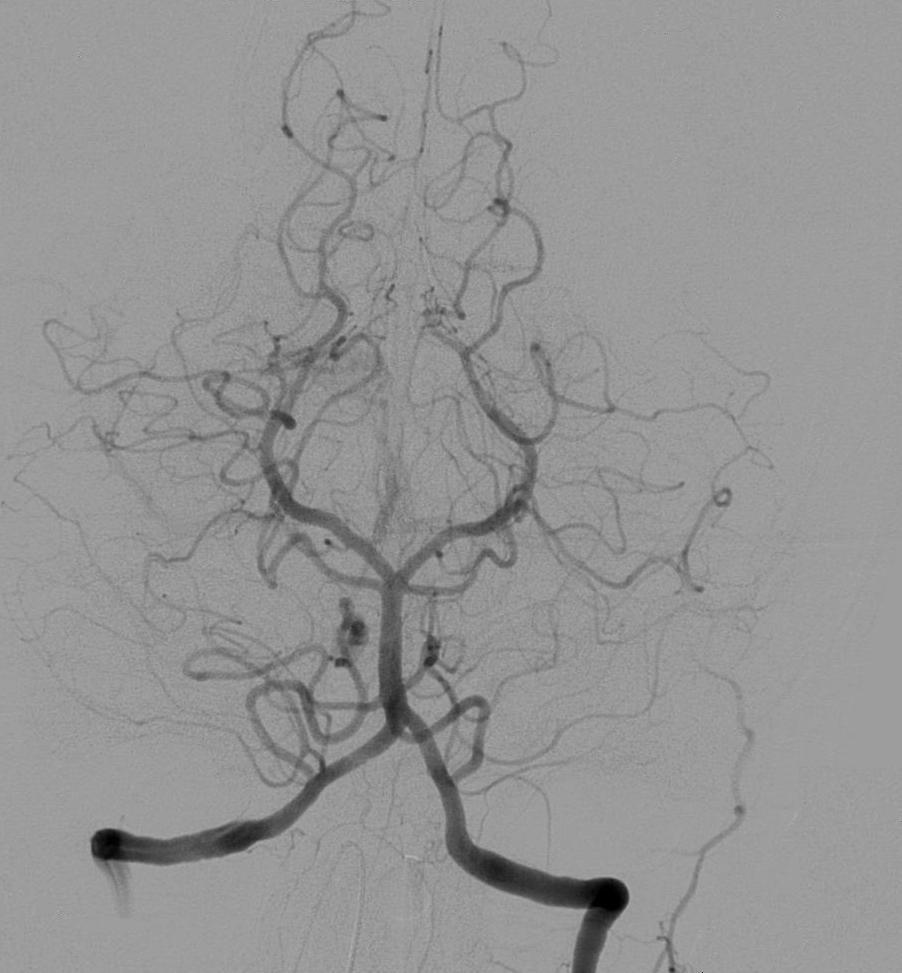
\includegraphics[scale=0.16]{figures/motivation/completion/angiogram.jpg}
		
	};
	\node at (current page.center) 
	    [
	    anchor=west,
	    xshift=-10mm,
	    yshift=0mm
	    ] 
	{
	
	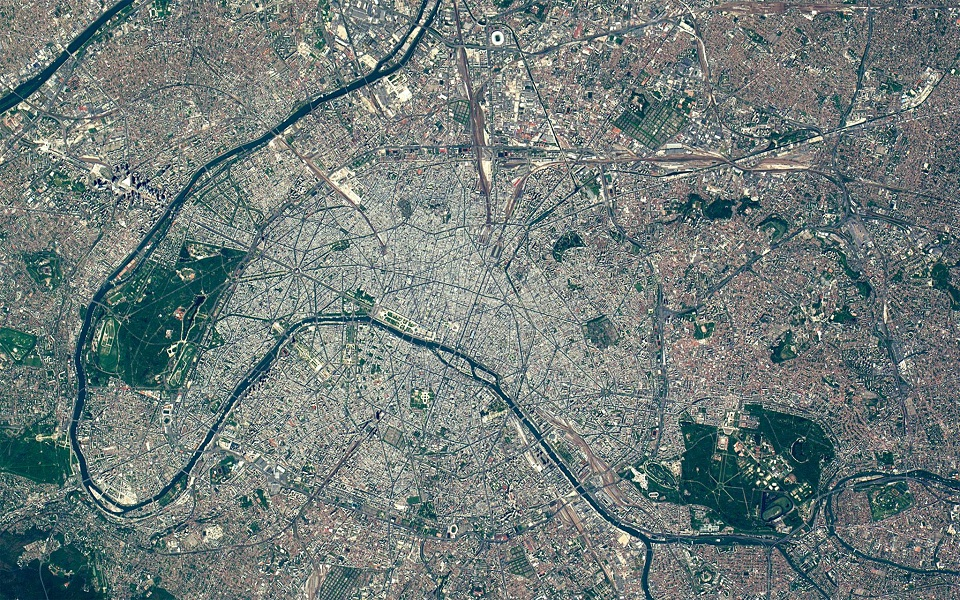
\includegraphics[scale=0.35]{figures/motivation/completion/paris-satellite-road.jpg}
		
	};	
	\end{tikzpicture}	
	\end{figure}	
	}	
\end{minipage}
\end{frame}

\begin{frame}
{Motivation}
{State-of-the-art}
\small
\textbf{Continuous setting}: Define the energy over the whole domain and minimize the elastica with respect the level-curves~(\mycite{chan02elasticainpainting}).
%
\begin{align*}
\int_{\Omega}{ \left(\alpha + \beta \nabla \cdot \left(\frac{\nabla f_{\vec{I}}}{\norm{\nabla f_{\vec{I}} }}\right) ^2 \right)\norm{\nabla f_{\vec{I}} }d\Omega}.
\end{align*}
%
\pause
\begin{itemize}
\item{Numerical instability: Fourth-order Euler-Lagrange equation.}
\item{Susceptible to bad local minimum.}
\end{itemize}
%
\pause
\vspace{0.5em}
\textbf{Discrete setting}:
\vspace{-1em}
\setlength\tabcolsep{3pt}
\begin{center}
\renewcommand{\arraystretch}{0.25}
\begin{tabular}{p{0.4\textwidth}p{0.6\textwidth}}
T-junctions matching & \multirow{2}{0.6\textwidth}{\footnotesize Fast algorithm, but limited to absolute value of curvature (polygonal solutions) and inpainting application.} \\
\mycite{masnou98inpainting} &\pause\\[3em]
Linear programming & \multirow{2}{0.6\textwidth}{\footnotesize Global formulation, but prohibitive running times even for small (thus unprecise) neighborhoods. Not suitable for digital sets.} \\
\mycite{schoenemann09linear} &\pause\\[3em]
Triple cliques & \multirow{2}{0.6\textwidth}{\footnotesize Global formulation, quadratic non-submodular energy. Limited precision due combinatorial explosion.} \\
\mycite{nieuwenhuis14efficient} &
\end{tabular}
\end{center}
\end{frame}

\begin{frame}
{Motivation}
{Goals}

Models based on the minimization of the elastica energy

\center
\begin{tabular}{lcc|c|}
& Continuous & Discrete & \textbf{Digital} \\
\hline
Numerical instability & \negative{Yes} & \positive{No} & \positive{No} \\
Suitable for digital sets & \negative{No} & \negative{No} & \positive{Yes} \\
Rounding issues & \negative{Yes} & \positive{No} & \positive{No} \\
Global formulation & \positive{Yes} & \positive{Yes} & \negative{No} \\
Contour completion & \negative{Partial} & \negative{Partial} & \positive{Extended} \\
Global optimum (Free elastica) & \negative{-} & \negative{-} & \positive{Yes}
\end{tabular}

%\vspace{2em}
%
%\begin{itemize}
%\item{Can we define an elastica-based model for image analysis using multigrid convergent estimators? \only<4>{\positive{Yes!}}} \pause
%\item{Can we recover the completion property of elastica? \only<4>{\positive{Yes!}}} \pause
%\item{Can we escape bad local minima? \only<4>{\positive{Yes!}}}
%\end{itemize}

\end{frame}



\begin{frame}
	{Outline}

\begin{enumerate}
	{\transparent{0.4}
	\item{Motivation}
	\begin{itemize}
		\item{Image analysis and geometric priors}
		\item{Elastica model and completion property}		
		\item{State-of-the-art}							
	\end{itemize}}
	\vspace{1em}
	\item{Contribution}
	\begin{itemize}
		\item{Digital sets and convergent estimators}		
		\item{Elastica minimization via graph-cuts}	
	\end{itemize}
	\vspace{1em}
	\item{Conclusion and perspectives}
\end{enumerate}
\end{frame}

\section{Digital sets and convergent estimators}

\begin{frame}
\huge
\center
Digital sets and convergent estimators
\vspace{2em}

\begin{minipage}{0.7\textwidth}
\normalsize
\center
\begin{itemize}
\item{Digital grid particularities and restrictions.}
\item{Multigrid convergence of geometric estimators.}
\end{itemize}
\end{minipage}

\end{frame}

\begin{frame}
{Digital sets and convergent estimators}
{Digital set peculiarities}

\begin{minipage}[t][0.35\textheight][t]{1\textwidth}

Where can we do better?

\begin{itemize}
\item{Most of models neglect the digital character of digital images and ignore the fact that geometric measurements (mainly those local as tangent and curvature) in such objects should be done with a definition of \emph{convergence} that is specific for digital shapes.}
\end{itemize}
\vspace{1em}

\end{minipage}
%
%
\begin{minipage}[t][0.65\textheight][t]{1\textwidth}
\only<2>{
\textbf{Exact sampling x digitization}
\center
\begin{tabular}{ccc}
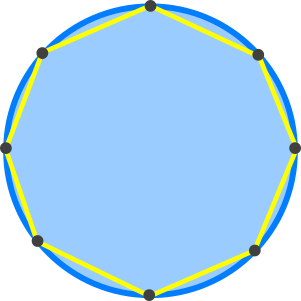
\includegraphics[scale=0.45]{figures/motivation/exact-sampling/sampling-0.png}&
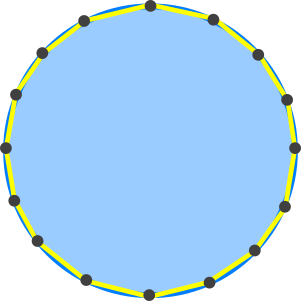
\includegraphics[scale=0.45]{figures/motivation/exact-sampling/sampling-1.png}&
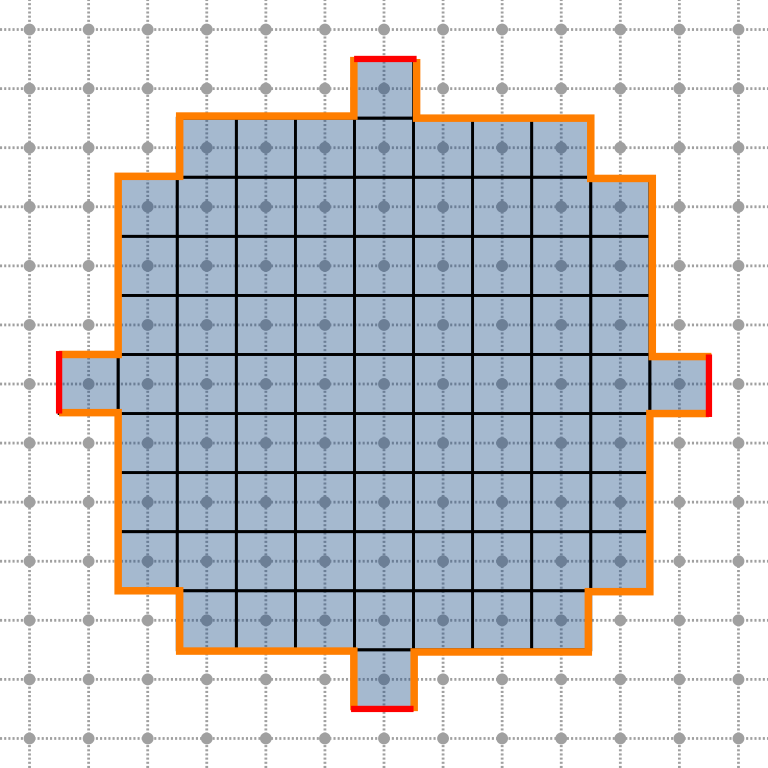
\includegraphics[scale=0.22]{figures/motivation/exact-sampling/digital-ball-perimeter.png}
\end{tabular}}%
\only<3>{
\textbf{Digitization ambiguity}

\begin{center}
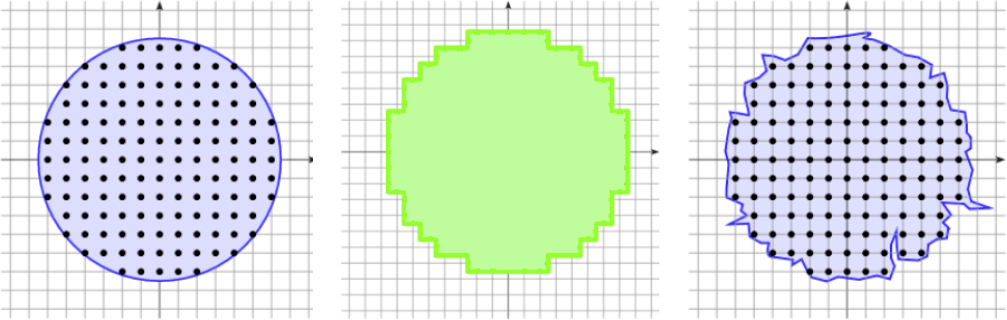
\includegraphics[scale=1]{figures/motivation/exact-sampling/ambiguity.png}
\end{center}}
\end{minipage}
\end{frame}

\begin{frame}
{Digital sets and convergent estimators}
{Multigrid convergent estimators}

\begin{definition}[Multigrid convergence]
	Let $\mathcal{X}$ be a family of shapes in $\mathbb{R}^n$ and $u$ a geometric quantity that is defined for every shape $X \in \mathcal{X}$. Further, let $D_h(X)$ denote the digitization of $X$ with grid step $h$.\\[1em]
	 The estimator $\hat{u}$ is multigrid convergent for $\mathcal{X}$ if and only if, for any $X \in \mathcal{X}$ there exists $h_X > 0$ such that for every $0< h < h_X$
	
	\begin{align*}
		| \hat{u}(D_h(X)) - u(X) | \leq \tau(h), \quad \text{with } \lim_{h\rightarrow 0}{\tau(h)} = 0.
	\end{align*}	
\end{definition}
%
\pause
%
Multigrid convergent estimator of area
\begin{align*}
	\widehat{Area(X)} = h^2|D_h(X)|.
\end{align*}
%
\end{frame}

\begin{frame}
{Motivation}
{Multigrid convergent estimators}

\footnotesize

\center
Disk of radius $5 (Area\approx78.54).$ 

\center
\begin{tabular}{ccc}
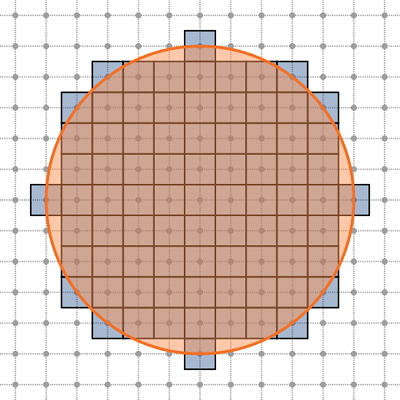
\includegraphics[scale=0.4]{figures/motivation/digital-geometric-estimators/multigrid/h1.png} &
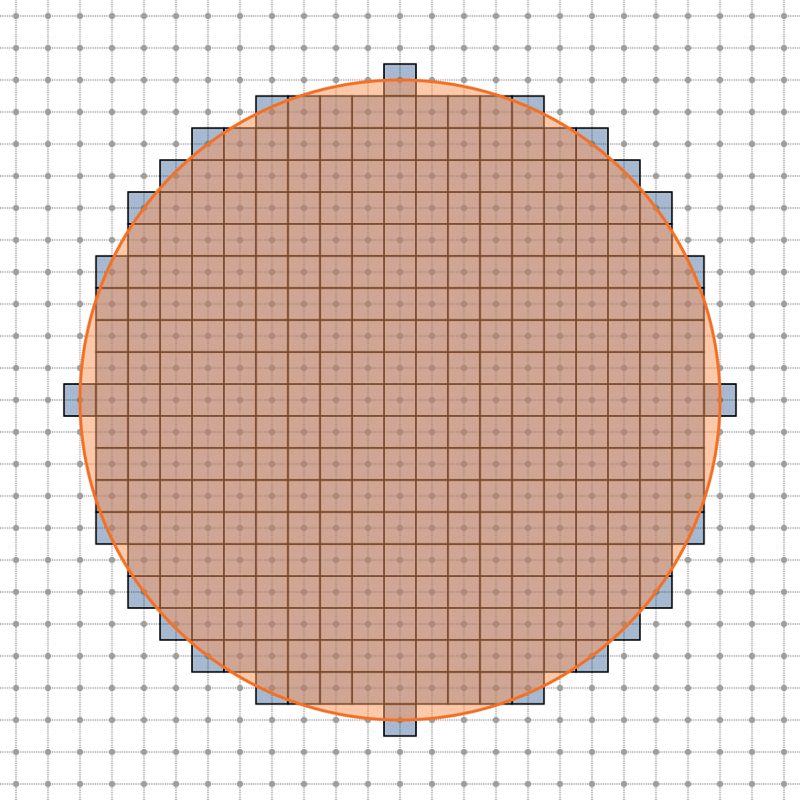
\includegraphics[scale=0.4]{figures/motivation/digital-geometric-estimators/multigrid/h05.png} &
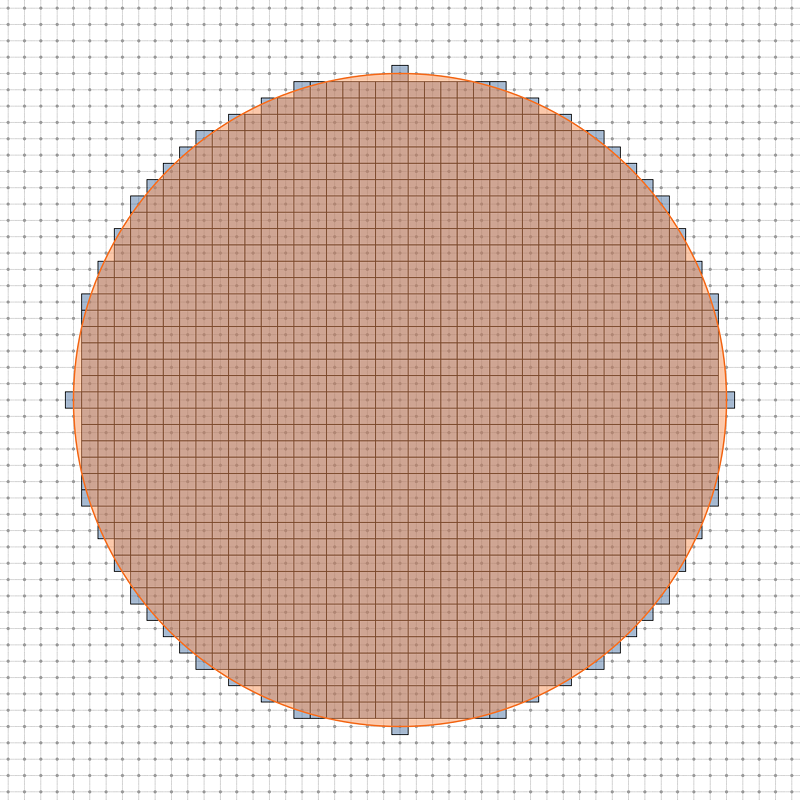
\includegraphics[scale=0.4]{figures/motivation/digital-geometric-estimators/multigrid/h025.png} \\
$h=1.0,\; \widehat{A}=81.$ & $h=\frac{1}{2},\; \hat{A}=79.25.$ & $h=\frac{1}{4},\; \hat{A}=78.56.$\\[1em]
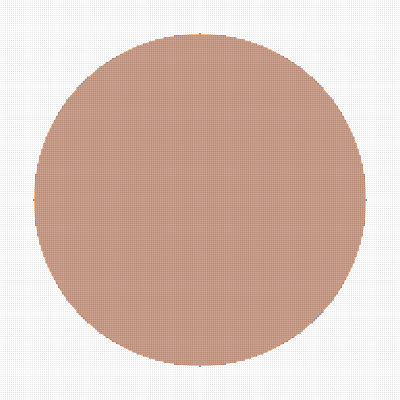
\includegraphics[scale=0.4]{figures/motivation/digital-geometric-estimators/multigrid/h00625.png} &

\includegraphics[scale=0.4]{figures/motivation/digital-geometric-estimators/multigrid/h003125.png} &

\includegraphics[scale=0.4]{figures/motivation/digital-geometric-estimators/multigrid/h003125.png} \\
$h=\frac{1}{16},\; \hat{A}=78.44.$ & $h=\frac{1}{32},\; \hat{A}=78.5.$ & $h=\frac{1}{64},\; \hat{A}=78.53.$
\end{tabular}

\end{frame}

% HT this frame does not compile
% \begin{frame}
% 	{Digital sets and convergent estimators}	
% 	{Multigrid convergent estimators}	
% %
% 	\begin{itemize}
% 		\onslide<1->{\item{Minimum Length Polygon (MLP)~\mycite{sloboda98approximation}}
% 		\begin{itemize}
% 			\item{Proved multigrid convergent for piecewise $3$-smooth convex shapes.}
% 		\end{itemize}}
% 		\onslide<3->{\vspace{2em}
% 		\item{Integral Invariant (II)~\mycite{coeurjolly13integral}}
% 		\begin{itemize}
% 			\item{Proved multigrid convergent for $C^2$ convex shapes with bounded curvature.}
% 		\end{itemize}}		
% 	\end{itemize}
	
% 	\onslide<2>{
% 	\begin{figure}
% 	\begin{tikzpicture}[overlay, remember picture] 
% 	\node at (current page.center) 
% 	    [
% 	    anchor=center,
% 	    xshift=0mm,
% 	    yshift=0mm
% 	    ] 
% 	{
	
% 	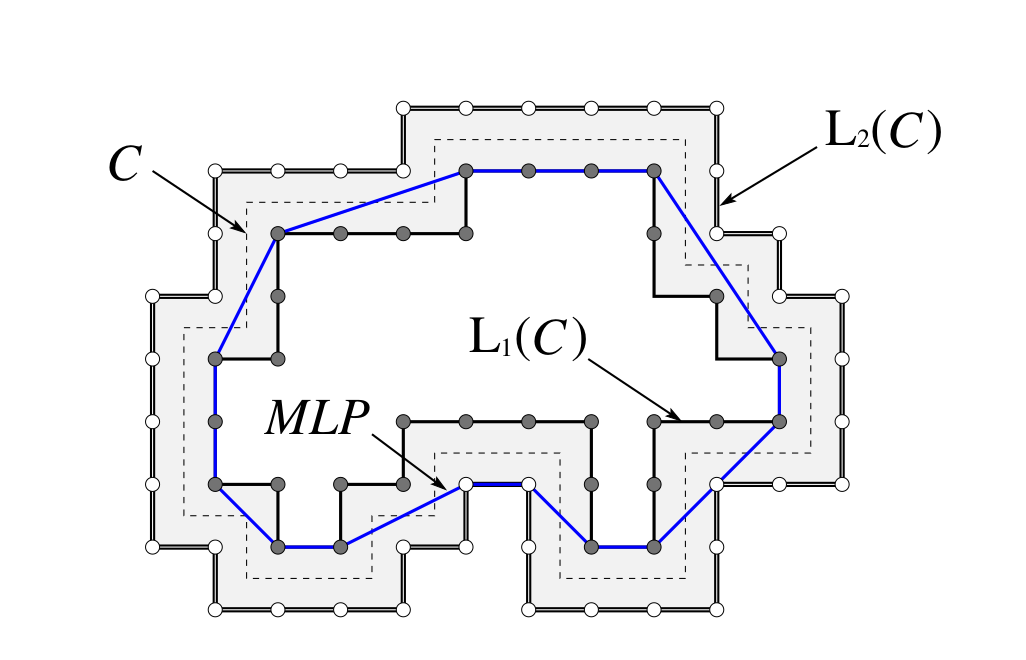
\includegraphics[scale=1.0]{figures/motivation/digital-geometric-estimators/mlp.png}
		
% 	};
% 	\end{tikzpicture}	
% 	\end{figure}	
% 	}
	
% 	\onslide<4->{
% 	\begin{figure}
% 	\begin{tikzpicture}[overlay, remember picture] 
% 	\node at (current page.center) 
% 	    [
% 	    anchor=center,
% 	    xshift=0mm,
% 	    yshift=0mm
% 	    ] 
% 	{
% 	\only<4>{
% 	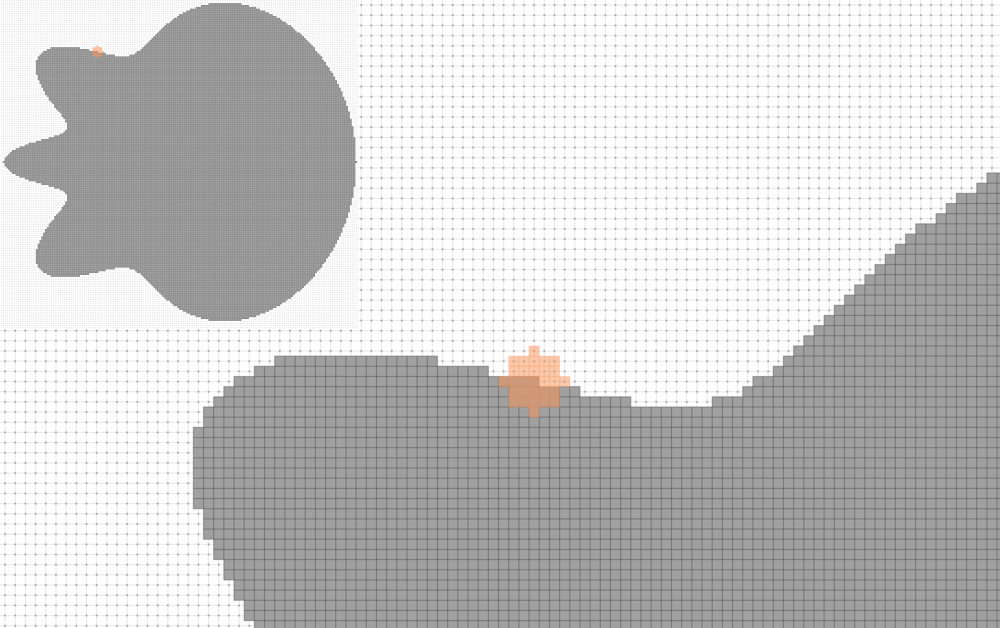
\includegraphics[scale=0.5]{figures/motivation/digital-geometric-estimators/ii/zoom/fr3-zoom.png}}%
% 	\only<5>{
% 	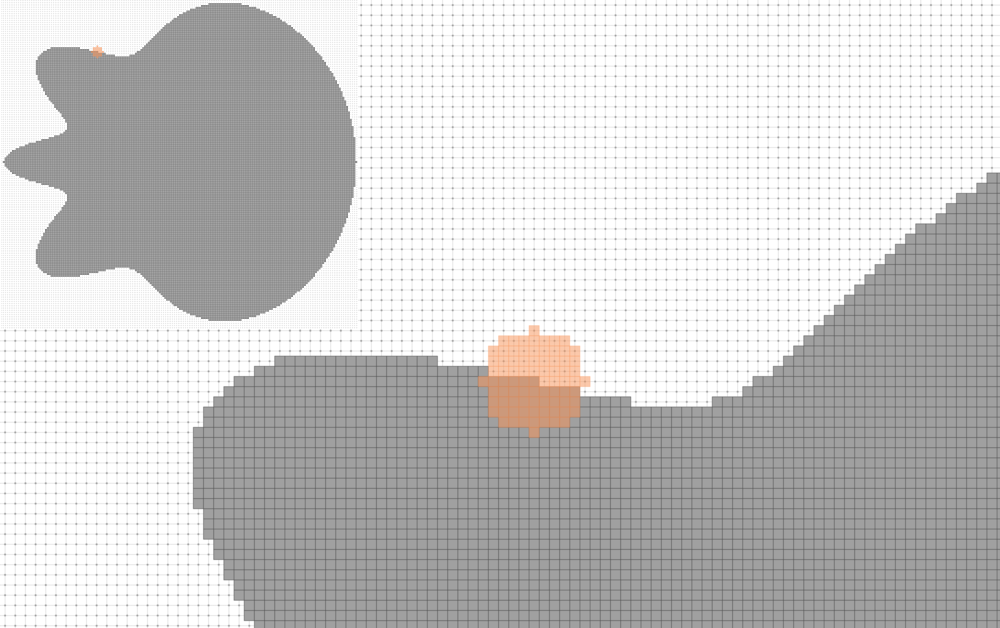
\includegraphics[scale=0.5]{figures/motivation/digital-geometric-estimators/ii/zoom/fr5-zoom.png}}%
		
% 	};
% 	\end{tikzpicture}	
% 	\end{figure}	
% 	}	

% 	\vspace{1.5em}

% 	\onslide<4->{
% 	\begin{align*}
% 		\hat{\kappa}(p) = \frac{3}{r^3}\left( \frac{\pi r^2}{2} - | B_r(p) \cap X | \right )
% 	\end{align*}}		
	
%     \end{frame}

 \begin{frame}
	{Digital sets and convergent estimators}	
	{Multigrid convergent estimators}	
%
	\begin{itemize}
		\item{Integral Invariant (II)~\mycite{coeurjolly13integral}}
		\begin{itemize}
			\item{Proved multigrid convergent for $C^2$ convex shapes with bounded curvature.}
		\end{itemize}		
	\end{itemize}
	
	
	\begin{figure}
	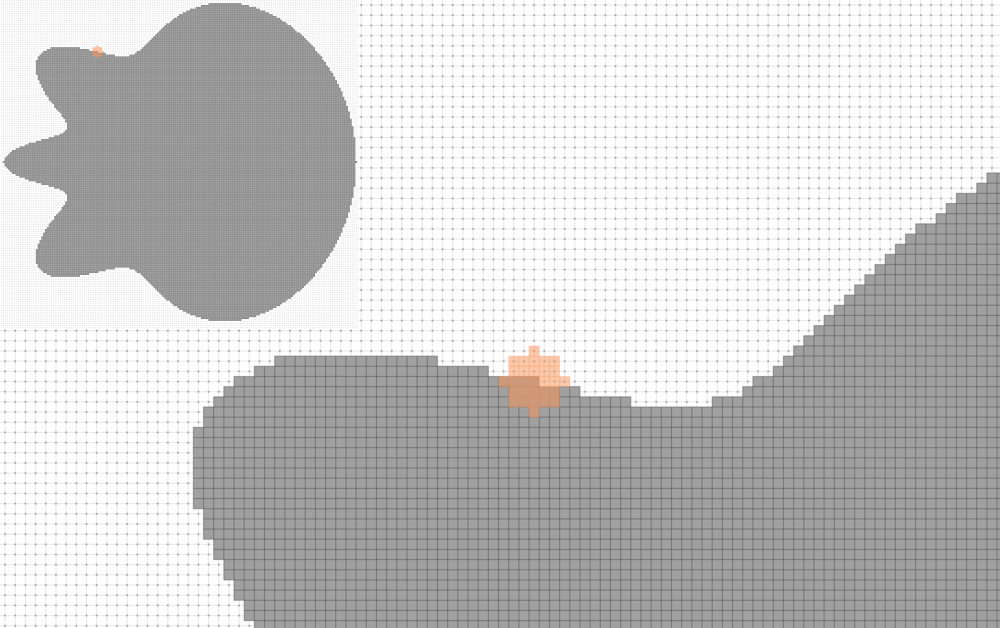
\includegraphics[scale=0.4]{figures/motivation/digital-geometric-estimators/ii/zoom/fr3-zoom.png}%		
	\end{figure}		

	\begin{align*}
		\hat{\kappa}(p) = \frac{3}{r^3}\left( \frac{\pi r^2}{2} - | B_r(p) \cap X | \right )
	\end{align*}
	
      \end{frame}

\begin{frame}
	{Digital sets and convergent estimators}	
	{Conclusion}	

	\begin{itemize}
		\item{Digital sets are ambiguous and are constrained to the digital grid.}\\[1em]
		\item{The multigrid convergence is an adapted definition of convergence for geometric estimation on digital sets.}\\[2em]\pause
		\item[]{\textbf{Can we construct optimization models using multigrid convergent estimators?}}
	\end{itemize}

\end{frame}
\section{Elastica minimization via graph-cuts}

\begin{frame}
\center
\huge
Elastica minimization via graph-cuts

\vspace{2em}

\begin{minipage}{0.7\textwidth}
\normalsize
\begin{itemize}
\item{Balance coefficient to estabilize curvature estimation.}
\item{Set up a graph whose minimum cut approximates the zero level set of the balance coefficient.}
\item{GraphFlow algorithm. Up to $10$x faster than FlipFlow.}
\end{itemize}
\end{minipage}

\end{frame}

\begin{frame}
{Non-submodular elastica}
{Balance coefficient}
\begin{minipage}{0.5\textwidth}
\center
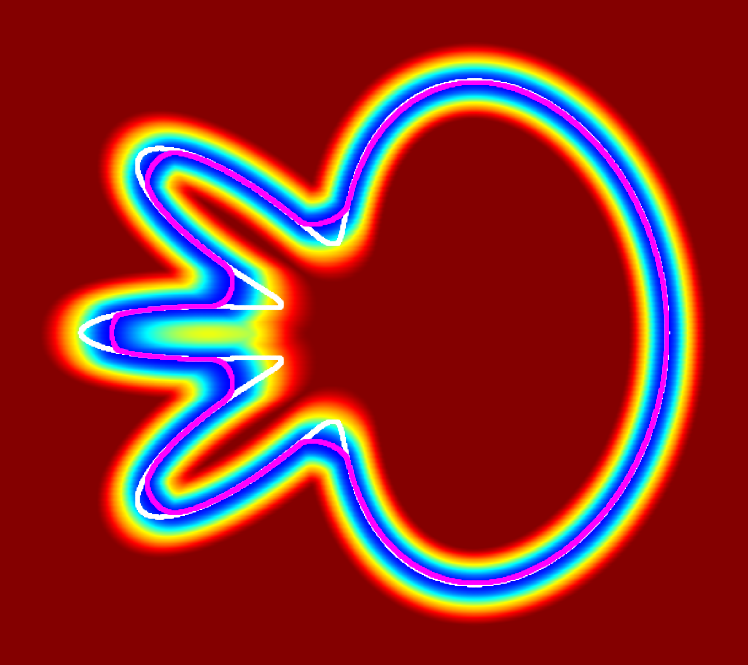
\includegraphics[scale=0.2]{figures/non-submodular-elastica/balance-coefficient-zero-level-set.png}
\end{minipage}
\begin{minipage}{0.49\textwidth}
\footnotesize
\begin{itemize}
\item{Balance coefficient}
\begin{align*}
u_r(D,p) &= \left( \frac{\pi r^2}{2} - |B_r(p) \cap D| \right)^2
\end{align*}
\item{White contour: contour of the shape}
\item{Pink contour: $\epsilon$-level set of the balance coefficient}
\end{itemize}
\end{minipage}
\end{frame}

\begin{frame}
{Elastica minimization via graph-cuts}
{Graph cut}
\center
\only<1>{
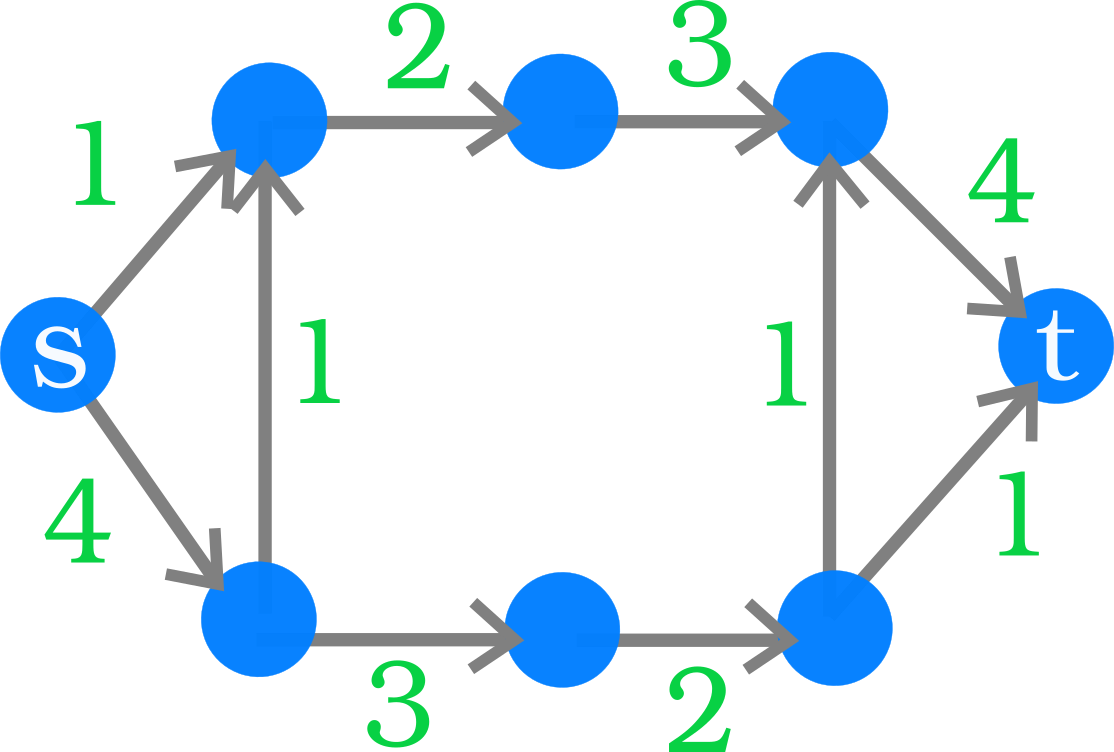
\includegraphics[scale=0.25]{figures/graphcut/cut-1.png}}%
\only<2>{
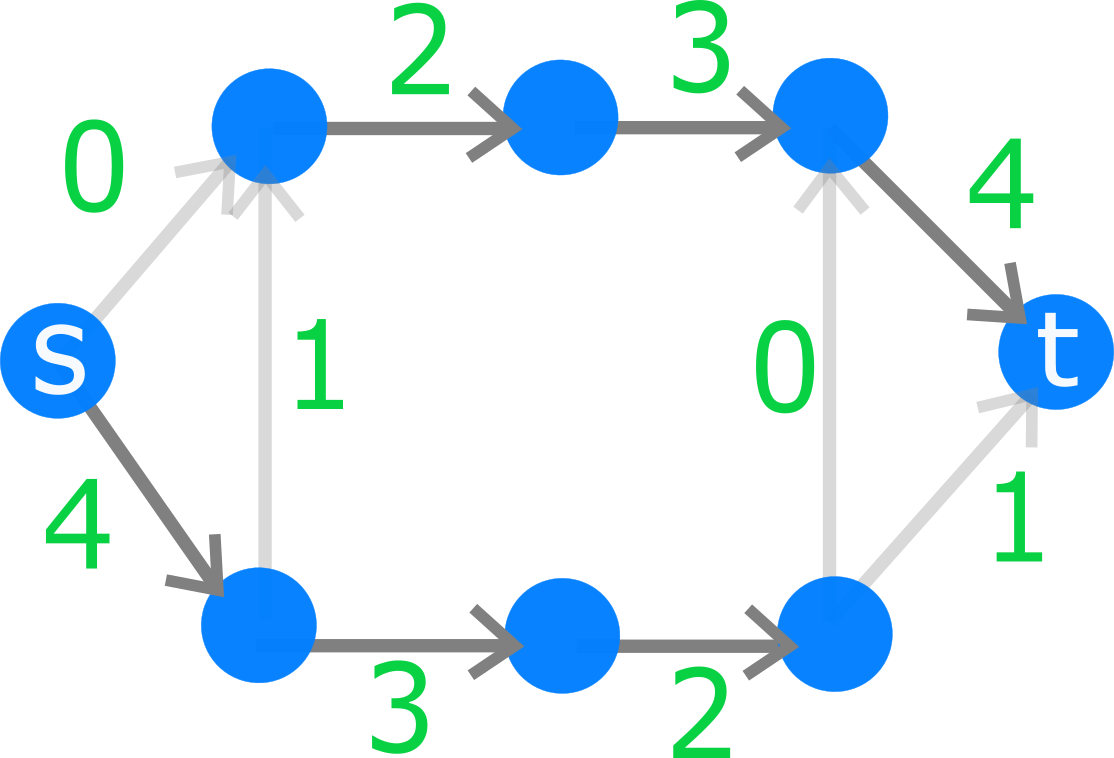
\includegraphics[scale=0.25]{figures/graphcut/cut-2.png}}%
\only<3>{
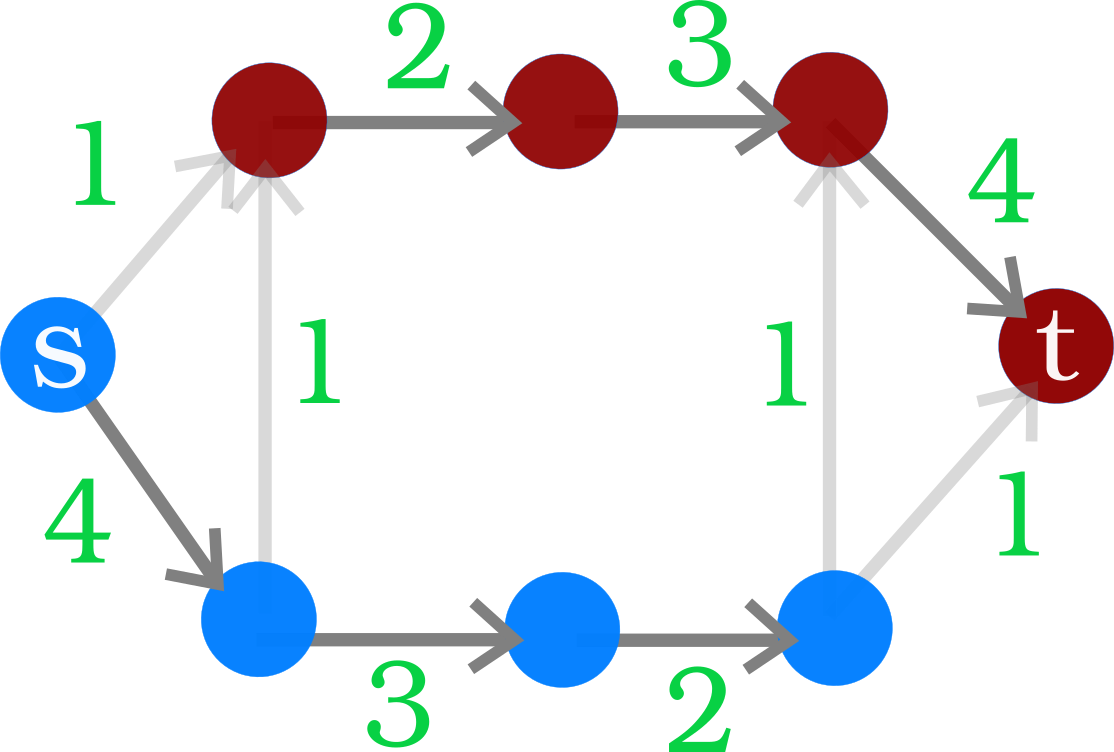
\includegraphics[scale=0.25]{figures/graphcut/cut-3.png}}%
\end{frame}


\begin{frame}
{Elastica minimization via graph-cuts}
{Building the graph}

\begin{minipage}{0.3\textwidth}
\only<1>{
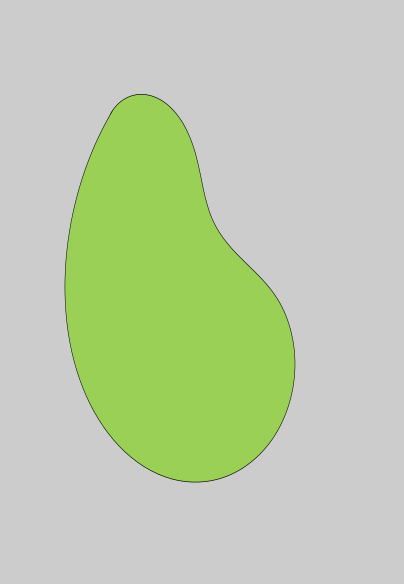
\includegraphics[scale=0.5]{figures/graphcut/graph-model-1.png}}%
\only<2-3>{
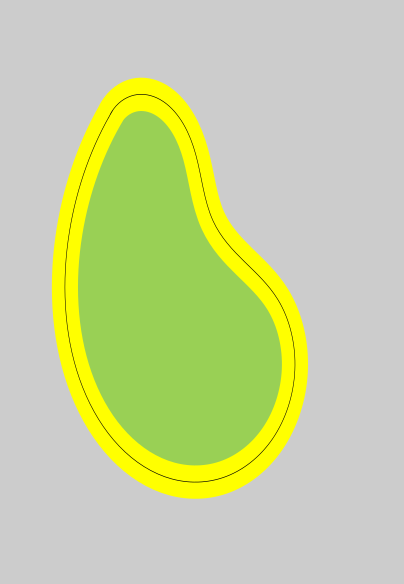
\includegraphics[scale=0.5]{figures/graphcut/graph-model-2.png}}%
\only<4->{
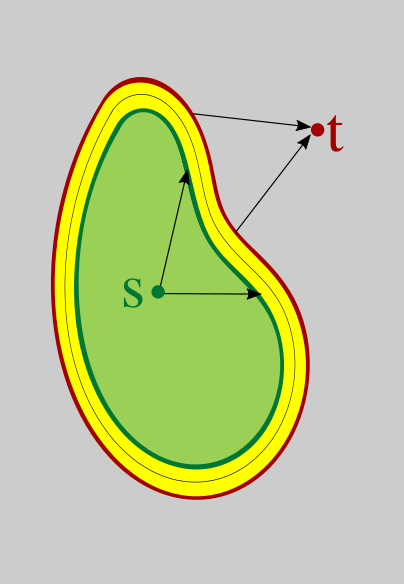
\includegraphics[scale=0.5]{figures/graphcut/graph-model-3.png}}%
\end{minipage}
%
%
\begin{minipage}{0.69\textwidth}
\footnotesize
\begin{itemize}
\onslide<2->{\item{Optimization band
\begin{align*}
%\only<2>{O_n(D) :=& \{ p \in D \; | \; -n \leq d_D(p) \leq n \} \\}
\only<2->{O(D) :=& \{ p \in D \; | \; -n \leq d_D(p) \leq n \} \\}
\onslide<3->{F(D) :=& D \setminus O(D)}
\end{align*}}}
\onslide<4->{\item{Graph $\mathcal{G}_D(\mathcal{V},\mathcal{E},c)$
\begin{align*}
\mathcal{V} &= \{ v_p \; | \; p \in O(D) \} \cup \{s,t\} \\
\highlight{6}{4,5,7-}{\mathcal{E}} &= \highlight{6}{4,5,7-}{\{ \{v_p,v_q\} \; | \; p,q \in O(D) \text{ and } q \in \mathcal{N}_4(p) \}} \cup \highlight{5}{4,6-}{\mathcal{E}_{st}} \\
\highlight{5}{4,6-}{\mathcal{E}_{st}} &= \highlight{5}{4,6-}{\{ (s,v_p), (v_p,t) \; | \; p \in O(D) \}}
\end{align*}}}
\onslide<7->{\item{Edge's weight
\begin{center}
\begin{tabular}{|c|c|}
\hline
\textbf{edge} $e$ & $\mathbf{c(e)}$\\
\hline
$\{v_p, v_q\}$ & $ \frac{1}{2}\left( u_r(D,p) + u_r(D,q)\right) $\\
\hline
$(s,v_p)$ & $M$\\
\hline
$(v_p, t)$ & $M$\\
\hline
\end{tabular}
\end{center}
}}
\onslide<8->{\item{Digital shape update
\begin{align*}
D^{(k+1)} &= F(D^{(k)}) + S^{(k)}
\end{align*}}}
\end{itemize}
\end{minipage}
\end{frame}
%
%
%
\begin{frame}
{Elastica minimization via graph-cuts}
{Shape evolution}

\begin{center}
$\alpha=1/8^2, \beta=1.$\\[1em]

\begin{tabular}{cc}
\includegraphics[scale=0.1]{figures/graphcut/no-neighborhood-flow-always-evolve/0.015625/triangle.png}\hspace{3em} &
\includegraphics[scale=0.08]{figures/graphcut/no-neighborhood-flow-always-evolve/0.015625/square.png}\\[1em]
\includegraphics[scale=0.12]{figures/graphcut/no-neighborhood-flow-always-evolve/0.015625/flower.png}\hspace{3em} &
\includegraphics[scale=0.12]{figures/graphcut/no-neighborhood-flow-always-evolve/0.015625/bean.png}
\end{tabular}
\end{center}

\onslide<2->{
\begin{itemize}
\item{What if we stop the evolution when elastica increases?}
\end{itemize}}

\end{frame}

\begin{frame}
{Elastica minimization via graph-cuts}
{Shape evolution}

\begin{center}
Stop if elastica increases $(\alpha=1/8^2,\beta=1)$\\[1em]

\begin{tabular}{cc}
\includegraphics[scale=0.1]{figures/graphcut/no-neighborhood-flow-always-improve/0.015625/triangle.png}\hspace{3em} &
\includegraphics[scale=0.08]{figures/graphcut/no-neighborhood-flow-always-improve/0.015625/square.png}\\[2em]
\includegraphics[scale=0.12]{figures/graphcut/no-neighborhood-flow-always-improve/0.015625/flower.png}\hspace{3em} &
\includegraphics[scale=0.12]{figures/graphcut/no-neighborhood-flow-always-improve/0.015625/bean.png}
\end{tabular}

\end{center}




\end{frame}

\begin{frame}
{Elastica minimization via graph-cuts}
{Shape evolution}

\begin{center}
Stop if elastica increases $(\alpha=1/22^2,\beta=1)$\\[1em]

\begin{tabular}{cc}
\includegraphics[scale=0.12]{figures/graphcut/no-neighborhood-flow-always-improve/0.0020661157/triangle.png}\hspace{3em} &
\includegraphics[scale=0.12]{figures/graphcut/no-neighborhood-flow-always-improve/0.0020661157/square.png}\\[2em]
\includegraphics[scale=0.12]{figures/graphcut/no-neighborhood-flow-always-improve/0.0020661157/flower.png}\hspace{3em} &
\includegraphics[scale=0.12]{figures/graphcut/no-neighborhood-flow-always-improve/0.0020661157/bean.png}
\end{tabular}

\end{center}




\end{frame}

\begin{frame}
{Elastica minimization via graph-cuts}
{The $a$-probe set}

\begin{definition}[$a$-probe set]
	Let $\Ds \subset \Omega \subset \mathbb{Z}^2$ a digital set and $a$ a natural number. The $a$-probe set of $\Ds$ is defined as
	\begin{align*}
		\mathcal{P}_a(\Ds) &= \Ds \cup \bigcup_{a' < a}{\Ds^{+a'} \cup \Ds^{-a'}},
	\end{align*}
	where $\Ds^{+a}$($\Ds^{-a}$) denotes a dilation(erosion) by a disk of radius $a$.
\end{definition}

\textbf{Candidate selection}
\[\begin{array}{l}
	sol(D^{(k)}) \longleftarrow \bigcup_{D' \in \mathcal{P}_a(D^{(k)})} \Big\{ F^{(k)} + S  \; | \; mincut(S,\mathcal{G}_{D'}) \Big\} 	
\end{array}
\]

\textbf{Candidate validation}
\[\begin{array}{l}
\Ds^{(k+1)} \longleftarrow \displaystyle \argmin_{ D' \in sol(D^{(k)}) }{ \hat{E}_{\vec{\theta}}(D')}
\end{array}
\]

\end{frame}

\begin{frame}
{Elastica minimization via graph-cuts}
{Shape evolution with $a$-probe set}

\center
\only<1>{Stop if elastica increases $(\alpha=1/22^2,\beta=1)$ \\[1em]}
\only<2>{Always update $(\alpha=1/22^2,\beta=1)$ \\[1em]}
\only<1>{
\begin{tabular}{cc}
\includegraphics[scale=0.12]{figures/graphcut/with-neighborhood-flow-always-improve/triangle.png}\hspace{3em} &
\includegraphics[scale=0.12]{figures/graphcut/with-neighborhood-flow-always-improve/square.png}\\[2em]
\includegraphics[scale=0.12]{figures/graphcut/with-neighborhood-flow-always-improve/flower.png}\hspace{3em} &
\includegraphics[scale=0.12]{figures/graphcut/with-neighborhood-flow-always-improve/bean.png}
\end{tabular}}
%
%
\only<2>{
\begin{tabular}{cc}
\includegraphics[scale=0.12]{figures/graphcut/with-neighborhood-flow/radius_16/triangle.png}\hspace{3em} &
\includegraphics[scale=0.12]{figures/graphcut/with-neighborhood-flow/radius_16/square.png}\\[2em]
\includegraphics[scale=0.12]{figures/graphcut/with-neighborhood-flow/radius_16/flower.png}\hspace{3em} &
\includegraphics[scale=0.12]{figures/graphcut/with-neighborhood-flow/radius_16/bean.png}
\end{tabular}}
\end{frame}

\begin{frame}
{Elastica minimization via graph-cuts}
{Shape evolution with $a$-probe set}

\begin{minipage}{0.25\textwidth}
\center
\includegraphics[scale=0.06]{figures/graphcut/with-neighborhood-flow/radius_16/triangle.png}\\[1em]
\includegraphics[scale=0.06]{figures/graphcut/with-neighborhood-flow/radius_16/square.png}\\[1em]
\includegraphics[scale=0.06]{figures/graphcut/with-neighborhood-flow/radius_16/flower.png}\\[1em]
\includegraphics[scale=0.06]{figures/graphcut/with-neighborhood-flow/radius_16/bean.png}
\end{minipage}%
%
%
\begin{minipage}{0.74\textwidth}
\center
\includegraphics[scale=0.18]{figures/graphcut/with-neighborhood-flow/plots/elastica.png}\\
\includegraphics[scale=0.18]{figures/graphcut/with-neighborhood-flow/plots/bars.png}
\end{minipage}
\end{frame}

\begin{frame}
{Elastica minimization via graph-cuts}
{Contour correction}

\begin{minipage}{0.5\textwidth}
\center
\only<1>{
\includegraphics[scale=0.45]{figures/graphcut/contour-correction/cat/gc-seg.png}

Initial segmentation

}%
\only<2>{
\includegraphics[scale=0.45]{figures/graphcut/contour-correction/vase/gc-seg.png}

Initial segmentation

}%
\only<3,4>{
\includegraphics[scale=0.4]{figures/graphcut/contour-correction/coala/gc-seg.png}

Initial segmentation

}%
\end{minipage}%
\begin{minipage}{0.5\textwidth}
\center
\only<1>{
\includegraphics[scale=0.45]{figures/graphcut/contour-correction/cat/corrected-seg.png}

$0.825s$ ($3$ it)

}%
\only<2>{\includegraphics[scale=0.45]{figures/graphcut/contour-correction/vase/corrected-seg.png}

$0.746s$ ($3$ it)

}%
\only<3>{\includegraphics[scale=0.4]{figures/graphcut/contour-correction/coala/5it.png}

$1.1s$ ($3$ it)

}%
\only<4>{\includegraphics[scale=0.4]{figures/graphcut/contour-correction/coala/30it.png}

$10s$ ($30$ it)

}%
\end{minipage}%

\end{frame}

\begin{frame}
{Elastica minimization via graph-cuts}
{Contour completion}

\begin{minipage}[t][0.47\textheight]{1\textwidth}
\center
\includegraphics[scale=0.28]{figures/graphcut/contour-completion/green-snake/gc-seg.png}

Initial segmentation

\end{minipage}
\vspace{1em}
\begin{minipage}[t][0.47\textheight]{1\textwidth}
\center
\includegraphics[scale=0.28]{figures/graphcut/contour-completion/green-snake/corrected-seg.png}

$17s$ ($62$ it)

\end{minipage}


\end{frame}

\section{Conclusion}

\begin{frame}
{Conclusion}
{Summary of models}

\onslide<1->{
\begin{table}[H]
\footnotesize
\centering
\begin{tabular}{r|ccccc}
\multirow{2}{*}{Model} & \multirow{2}{*}{Implementation} & Running & Free & Constrained & Image\\
& & time & elastica & elastica & term\\
\hline
LocalSearch & medium & \negative{slow} & \positive{yes(\textbf{opt})} & \positive{yes} & \negative{no}\\
FlipFlow  & \negative{hard} & acceptable & \positive{yes} & \negative{no} & \positive{yes}\\
( BalanceFlow ) & medium & acceptable & \positive{yes} & \negative{no} & \positive{yes}\\
GraphFlow  & \positive{easy} & \positive{fast} & \positive{yes(\textbf{opt})} & \negative{no} & \positive{yes}
\end{tabular}
\caption{\textbf{Models summary.} The qualitative attributes are relative, e.g., the GraphFlow presents the lowest running time while LocalSearch presents the highest.}
\end{table}}

\onslide<2->{
\begin{figure}
\center
\captionsetup{type=table}
\footnotesize
\begin{tabular}{|l|c|c|c|c|c|}
\hline
& Pixels & LocalSearch & FlipFlow & BalanceFlow & GraphFlow \\
\hline
Triangle & 8315 & \negative{4.8s/it} & 0.4s/it & 0.38s/it & \positive{0.14s/it}\\
Square & 12769 & \negative{2s/it} & 0.51s/it & 0.47s/it & \positive{0.12s/it}\\
Ellipse  & 10038 & \negative{3.1s/it} & 0.64s/it & 0.57s/it & \positive{0.1s/it} \\
Flower & 26321 & \negative{12.3s/it} & 1.23s/it & 0.94s/it & \positive{0.14s/it}\\
Bean  & 25130 & \negative{6.4s/it} & 1.2s/it & 1.17s/it & \positive{0.16s/it}\\
\hline
\end{tabular}
\caption{\textbf{Free elastica running times.} Running time and input size for the free elastica experiment.}
\end{figure}}

\end{frame}

\begin{frame}
{Conclusion}
{Summary of models}

\begin{itemize}
\item{We achieved global optimum elastica with a digital model.}
\pause
\item{GraphFlow is extendable (suitable for data terms) and our fastest model.}
\pause
\item{Contour completion is achieved in some cases.}
\pause
\end{itemize}

\textbf{Pros}
\begin{itemize}
\item{Topology is flexible.}
\pause
\item{Easily parallelizable.}
\pause
\item{Flexibility of neighborhood of shapes.}
\pause
\end{itemize}

\textbf{Cons}
\begin{itemize}
\item{Susceptible to bad local minimum (we can escape it with a proper definition of the neighborhood).}
\end{itemize}

\end{frame}

\begin{frame}
{Conclusion}
{Perspectives}

\begin{itemize}
\item{\textbf{GraphFlow and perimeter}: enrich the cost function of GraphFlow with the weights defined in~\mycite{boykov03geodesics}. }
\pause
\item{\textbf{Different neighborhoods}: random, linear extension.}
\pause
\item{\textbf{Dynamic radius}: use the parameter free Maximal Digital Circular Arcs estimator of curvature to adapt the estimation disk radius to use.}
\pause
\item{\textbf{Multiresolution}: Improve running time; or improve estimator precision.}
\pause
\item{\textbf{Image analysis applications}: Make an objective comparison of our method and competitive ones (e.g. study quantitative measurements such as the ratio of inflexion points for the contour correction application) .}
\pause
\item{\textbf{Global formulation and multigrid convergent estimators}: Do there exist a practicable model for elastica?}
\end{itemize}

\end{frame}

\begin{frame}
\huge
\center
Thank you!
\end{frame}


\begin{frame}[allowframebreaks]
    \frametitle{References}	
    \printbibliography
\end{frame}


\end{document}